% \section{Approach}

% \section{Research methods}
% \section{DSRM}

% \begin{figure}[ht]
% 	\centering
% 	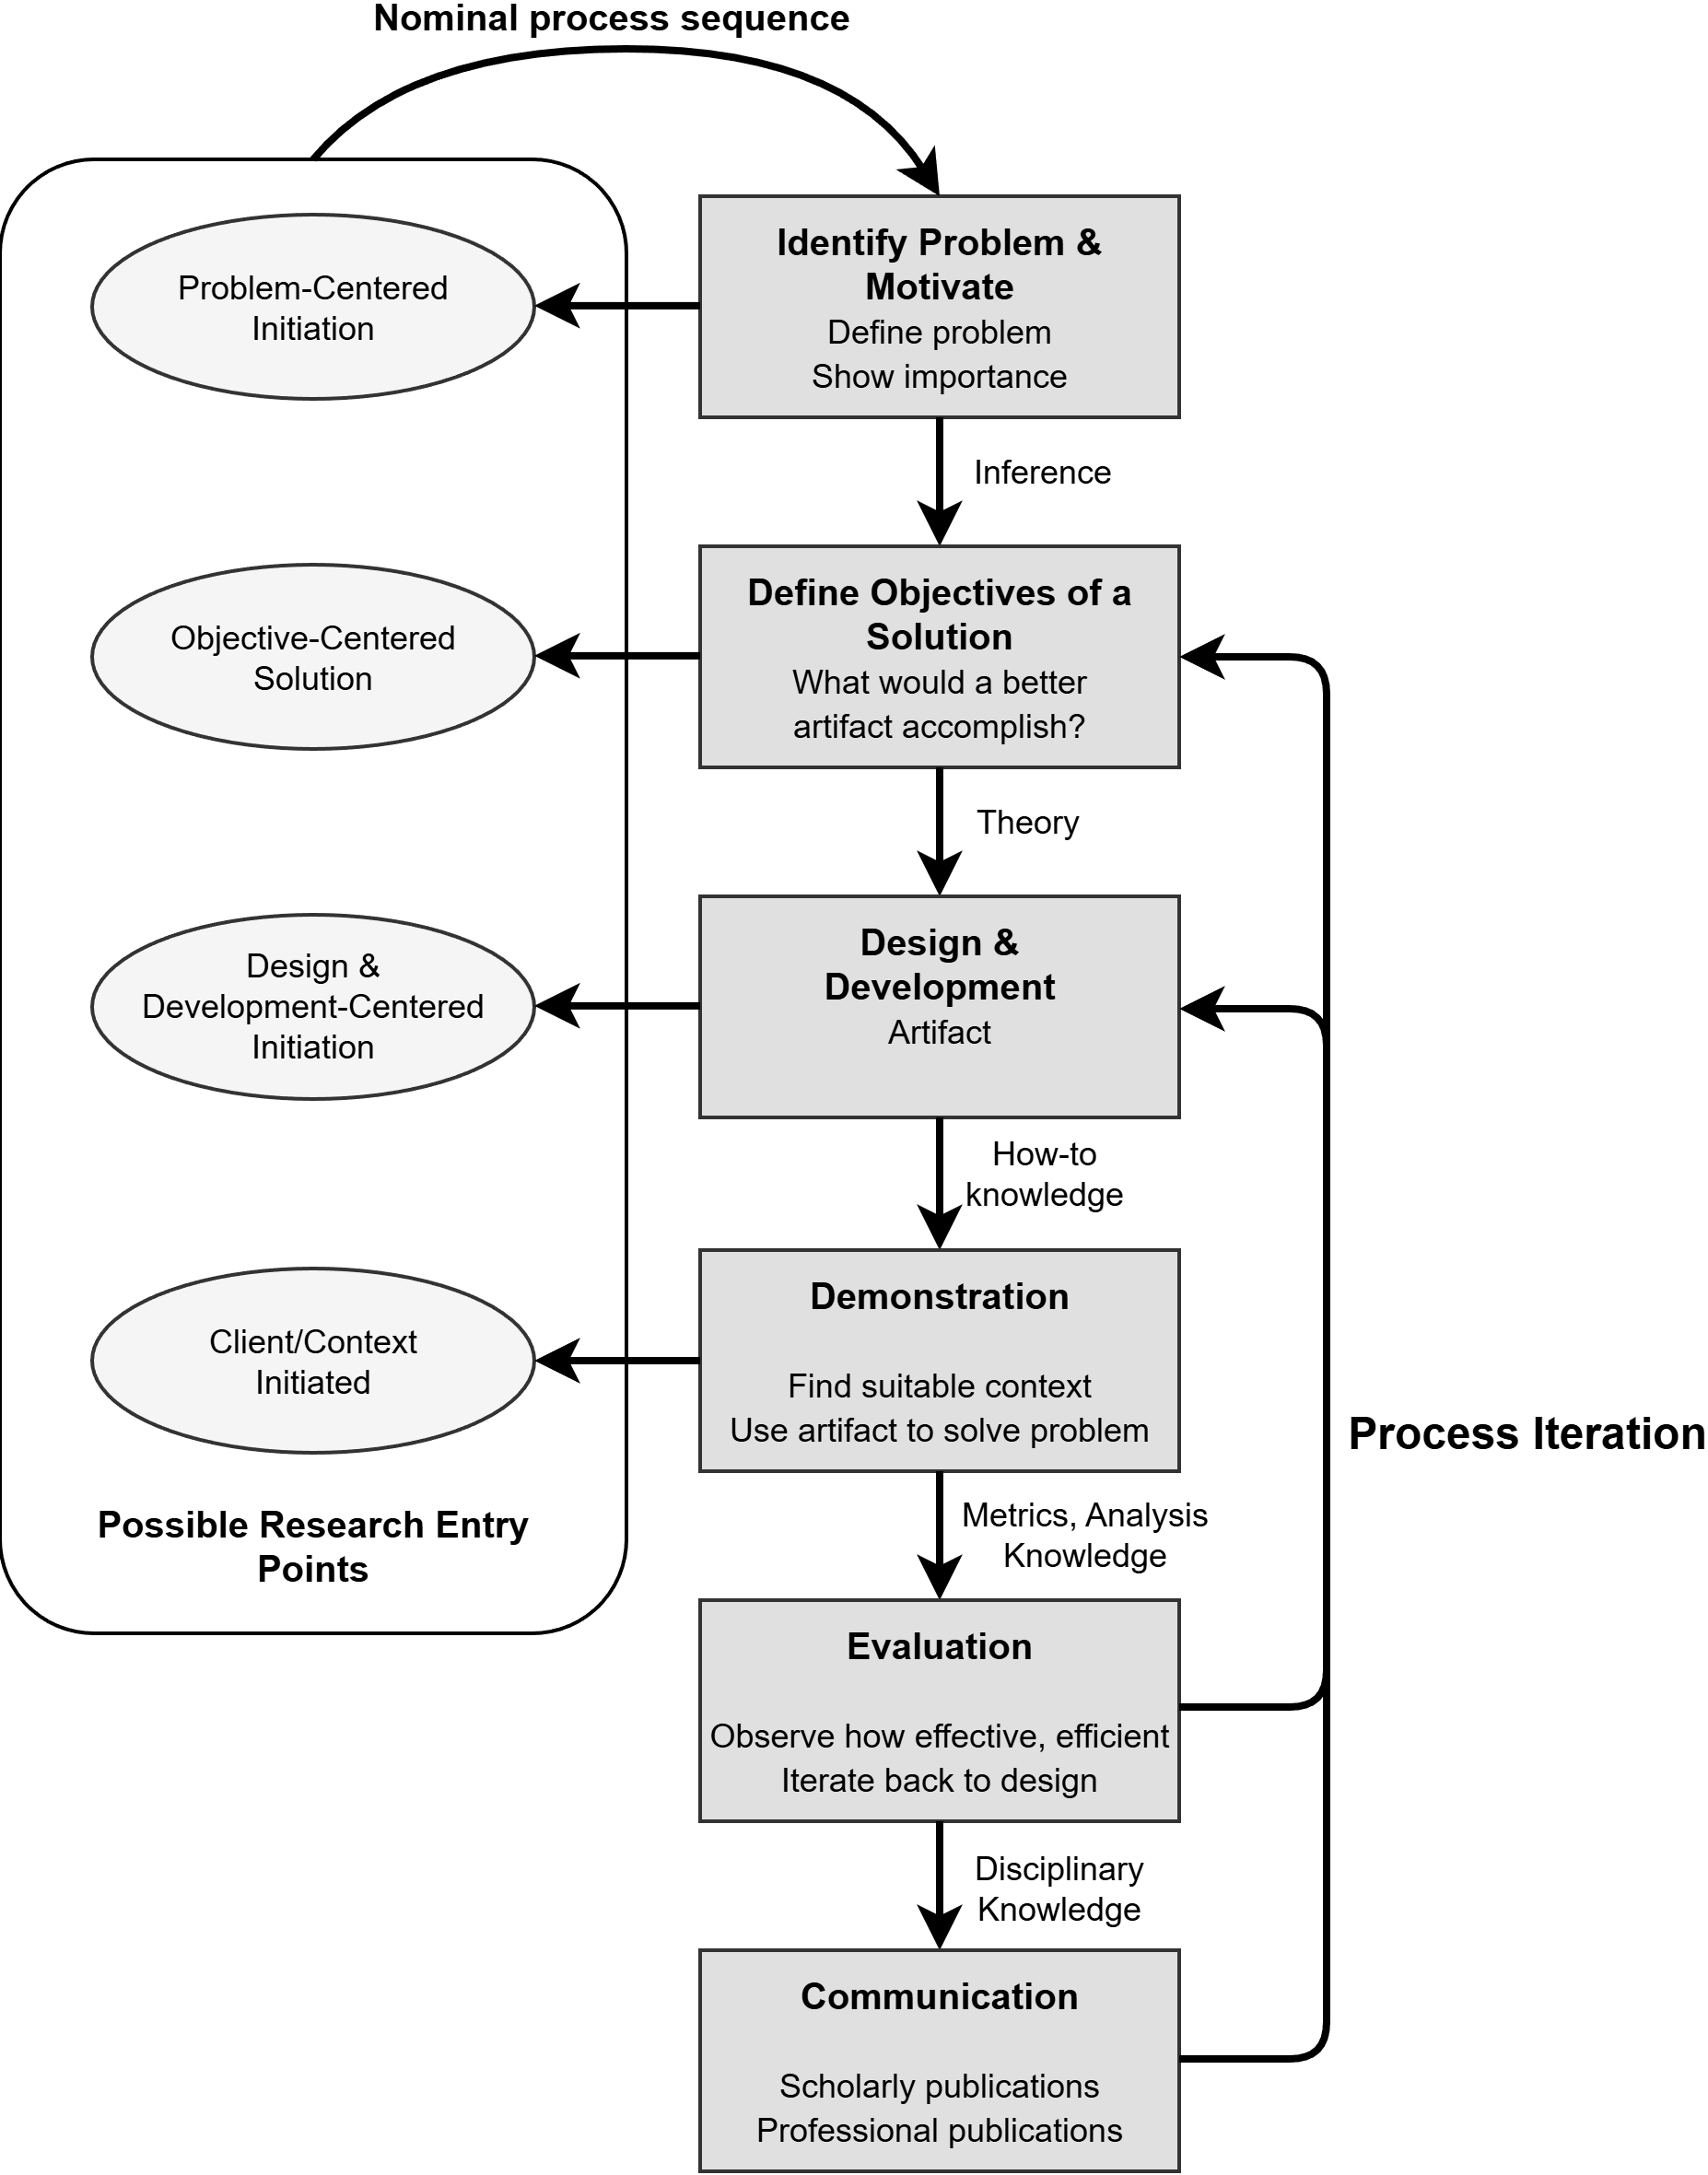
\includegraphics[width=0.95\linewidth]{figures/DSRM_Process_Model.png}
% 	\caption{DSRM Process Model \citep{peffersDesignScienceResearch2007}}
% 	\label{fig:DSRM_Process_Model}
% \end{figure}

% Problem centered initiation: Reproducibility in legacy software development projects is hard to achieve without containerization.
% So how can it be achieved with containerization?


% \begin{itemize}
% 	\item \textbf{Problem Identification:} Recognizing the need for modernization in legacy software development.
% 	\item \textbf{Objectives of a Solution:} Defining the goals for a containerized development environment.
% 	\item \textbf{Design and Development:} Developing a prototype that integrates VS Code and Docker.
% 	\item \textbf{Demonstration:} Applying the prototype in real-world scenarios.
% 	\item \textbf{Evaluation:} Assessing the effectiveness and efficiency of the solution.
% 	\item \textbf{Communication:} Presenting the findings and their implications for the field.
% \end{itemize}

% \section{Experimental design}

\chapter{Prototype Architecture}
\label{ch:prototype_architecture}

This chapter introduces the architecture of the prototype developed for this thesis, focusing on modernizing legacy software development workflows through containerization and infrastructure automation.
The prototype serves as a practical exploration of the theoretical concepts discussed in the fundamentals chapter and provides a framework for analyzing the impact of containerization on development productivity and reproducibility.
To describe the architecture systematically, the 4+1 Architectural View Model presented by \citet{kruchten4+1ViewModel1995} is utilized, as illustrated in Figure \ref{fig:4+1-view-model}.
This methodological approach provides a robust framework for presenting software-intensive system architectures through multiple concurrent views, addressing both functional and non-functional requirements across five distinct perspectives.

\begin{figure}[ht]
	\centering
	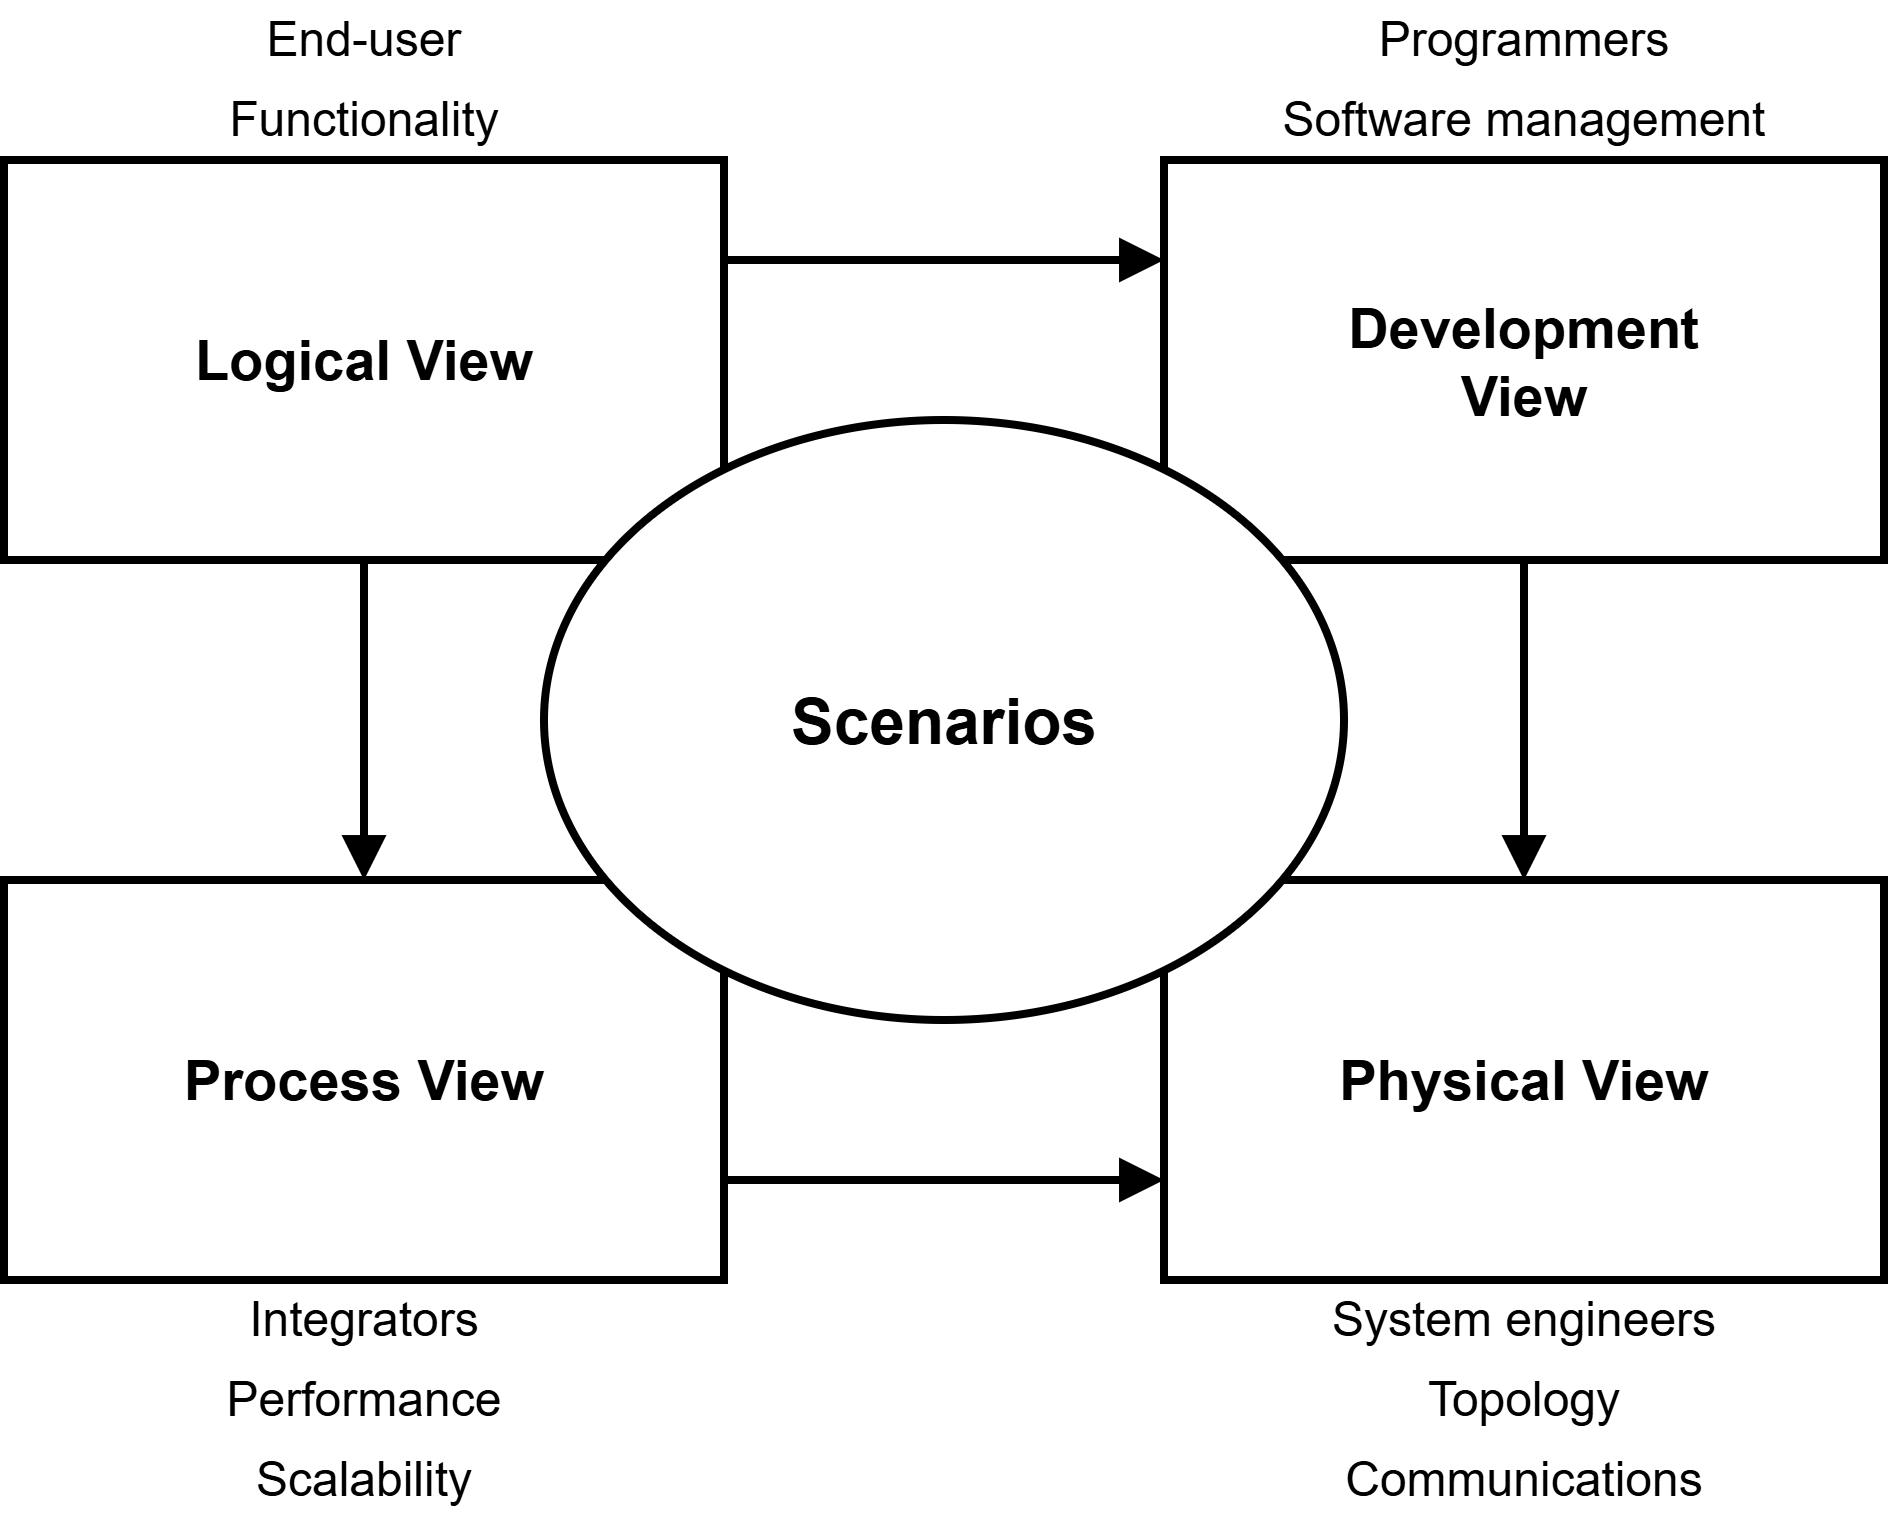
\includegraphics[width=0.9\linewidth]{figures/4+1-view-model.png}
	\caption{The 4+1 View Model of Software Architecture (adapted from \cite{kruchten4+1ViewModel1995})}
	\label{fig:4+1-view-model}
\end{figure}

The prototype addresses the fundamental challenge of environment consistency in legacy software development by providing automated, reproducible development environments across multiple platforms \citep{chamberlainUsingDockerSupport2014, citoUsingDockerContainers2016}.
Unlike traditional manual setup processes that are prone to configuration drift and environmental inconsistencies, this prototype implements infrastructure-as-code principles to ensure deterministic and version-controlled development environments \citep{humbleContinuousDeliveryReliable2011}.

The prototype is developed and evaluated in the context of WinCC Open Architecture (WinCC OA), a \ac{scada} software system with a codebase spanning over 30 years and actively maintained under continuous development.
The software, primarily written in C++, utilizes CMake as its build system generator, with Windows and Linux as the supported target platforms.
The transition to Git for source code management several years ago marked a significant shift in the development process, accompanied by the introduction of automated server builds for the target platforms through Jenkins.

The default working environment for WinCC OA developers is Windows, raising issues in ensuring code compatibility and successful builds on Linux, which historically relied on server builds for validation.
This prototype addresses these challenges through standardized containerized development environments that enable developers to build and test on both target platforms regardless of their host operating system.

\section{Logical Architecture}

The Logical View focuses on the functional requirements and structural organization of the prototype system.
This section describes the core functionality the system must provide, the architectural organization of functional components, and the interface design enabling seamless integration across different development workflows \citep{kruchten4+1ViewModel1995}.

\subsection{Functional Requirements}

The prototype application fulfills four fundamental requirements that address critical challenges in legacy software development modernization.

The primary requirement involves \textbf{automated environment provisioning} across heterogeneous platforms \citep{boettigerIntroductionDockerReproducible2015}.
The system must provide consistent development environments for both Windows and Linux platforms, eliminating manual configuration steps that introduce variability and human error \citep{hungGUIdockUsingDocker2016}.
For Windows environments, this involves utilizing pre-existing virtual machine templates with pre-configured development tools, compilers, and dependencies that developers can clone and deploy locally.
Automated VM template creation using tools such as HashiCorp Packer, while conceptually similar to container image building, introduces significantly higher complexity due to longer build times, larger artifact sizes, and platform-specific hypervisor requirements; therefore, automated VM template generation is considered out of scope for this prototype, with the assumption that suitable templates are maintained and distributed through organizational processes.
For Linux environments, this encompasses building optimized container images that encapsulate complete development toolchains while maintaining minimal resource footprints using Docker multi-stage builds \citep{merkelDockerLightweightLinux2014}.

The second major requirement addresses \textbf{cross-platform build system standardization} \citep{gygiCppBuildLargeScaleAutomatic2021}.
The prototype must provide unified build configurations that produce consistent results regardless of the underlying host operating system or deployment target.
This functionality ensures that developers working on different platforms can achieve identical build outputs, eliminating the common "works on my machine" problem that plagues legacy software projects \citep{pengReproducibleResearchComputational2011}.
The system accomplishes this through standardized CMake preset configurations that abstract platform-specific details while maintaining full control over compilation parameters.

The third requirement focuses on \textbf{developer experience optimization} through seamless IDE integration.
The prototype provides custom VS Code commands and configurations that abstract complex containerization and virtualization workflows into simple, accessible operations.
This integration enables developers to leverage advanced environment isolation benefits without requiring deep expertise in container or virtualization technologies, thereby reducing adoption barriers and improving overall productivity \citep{danilovVSCodeDockerized2022, luDevelopmentDockerContainers2018}.

The fourth requirement encompasses \textbf{comprehensive performance measurement} capabilities.
The prototype must capture quantitative metrics across different development workflows, including environment setup times, build performance (cold and warm builds), test execution performance, and resource utilization patterns.
These measurements enable systematic comparison between virtualized and containerized development approaches to inform architecture decisions.

\subsection{Component Architecture}

The logical architecture organizes the prototype system into seven major architectural components representing high-level functional groupings within the development environment modernization domain.
This component-based decomposition, following Kruchten's approach for larger systems \citep{kruchten4+1ViewModel1995}, addresses functional requirements at an architectural level.

Figure \ref{fig:logical-components} illustrates the component organization and their primary relationships.

\begin{figure}[ht!]
	\centering
	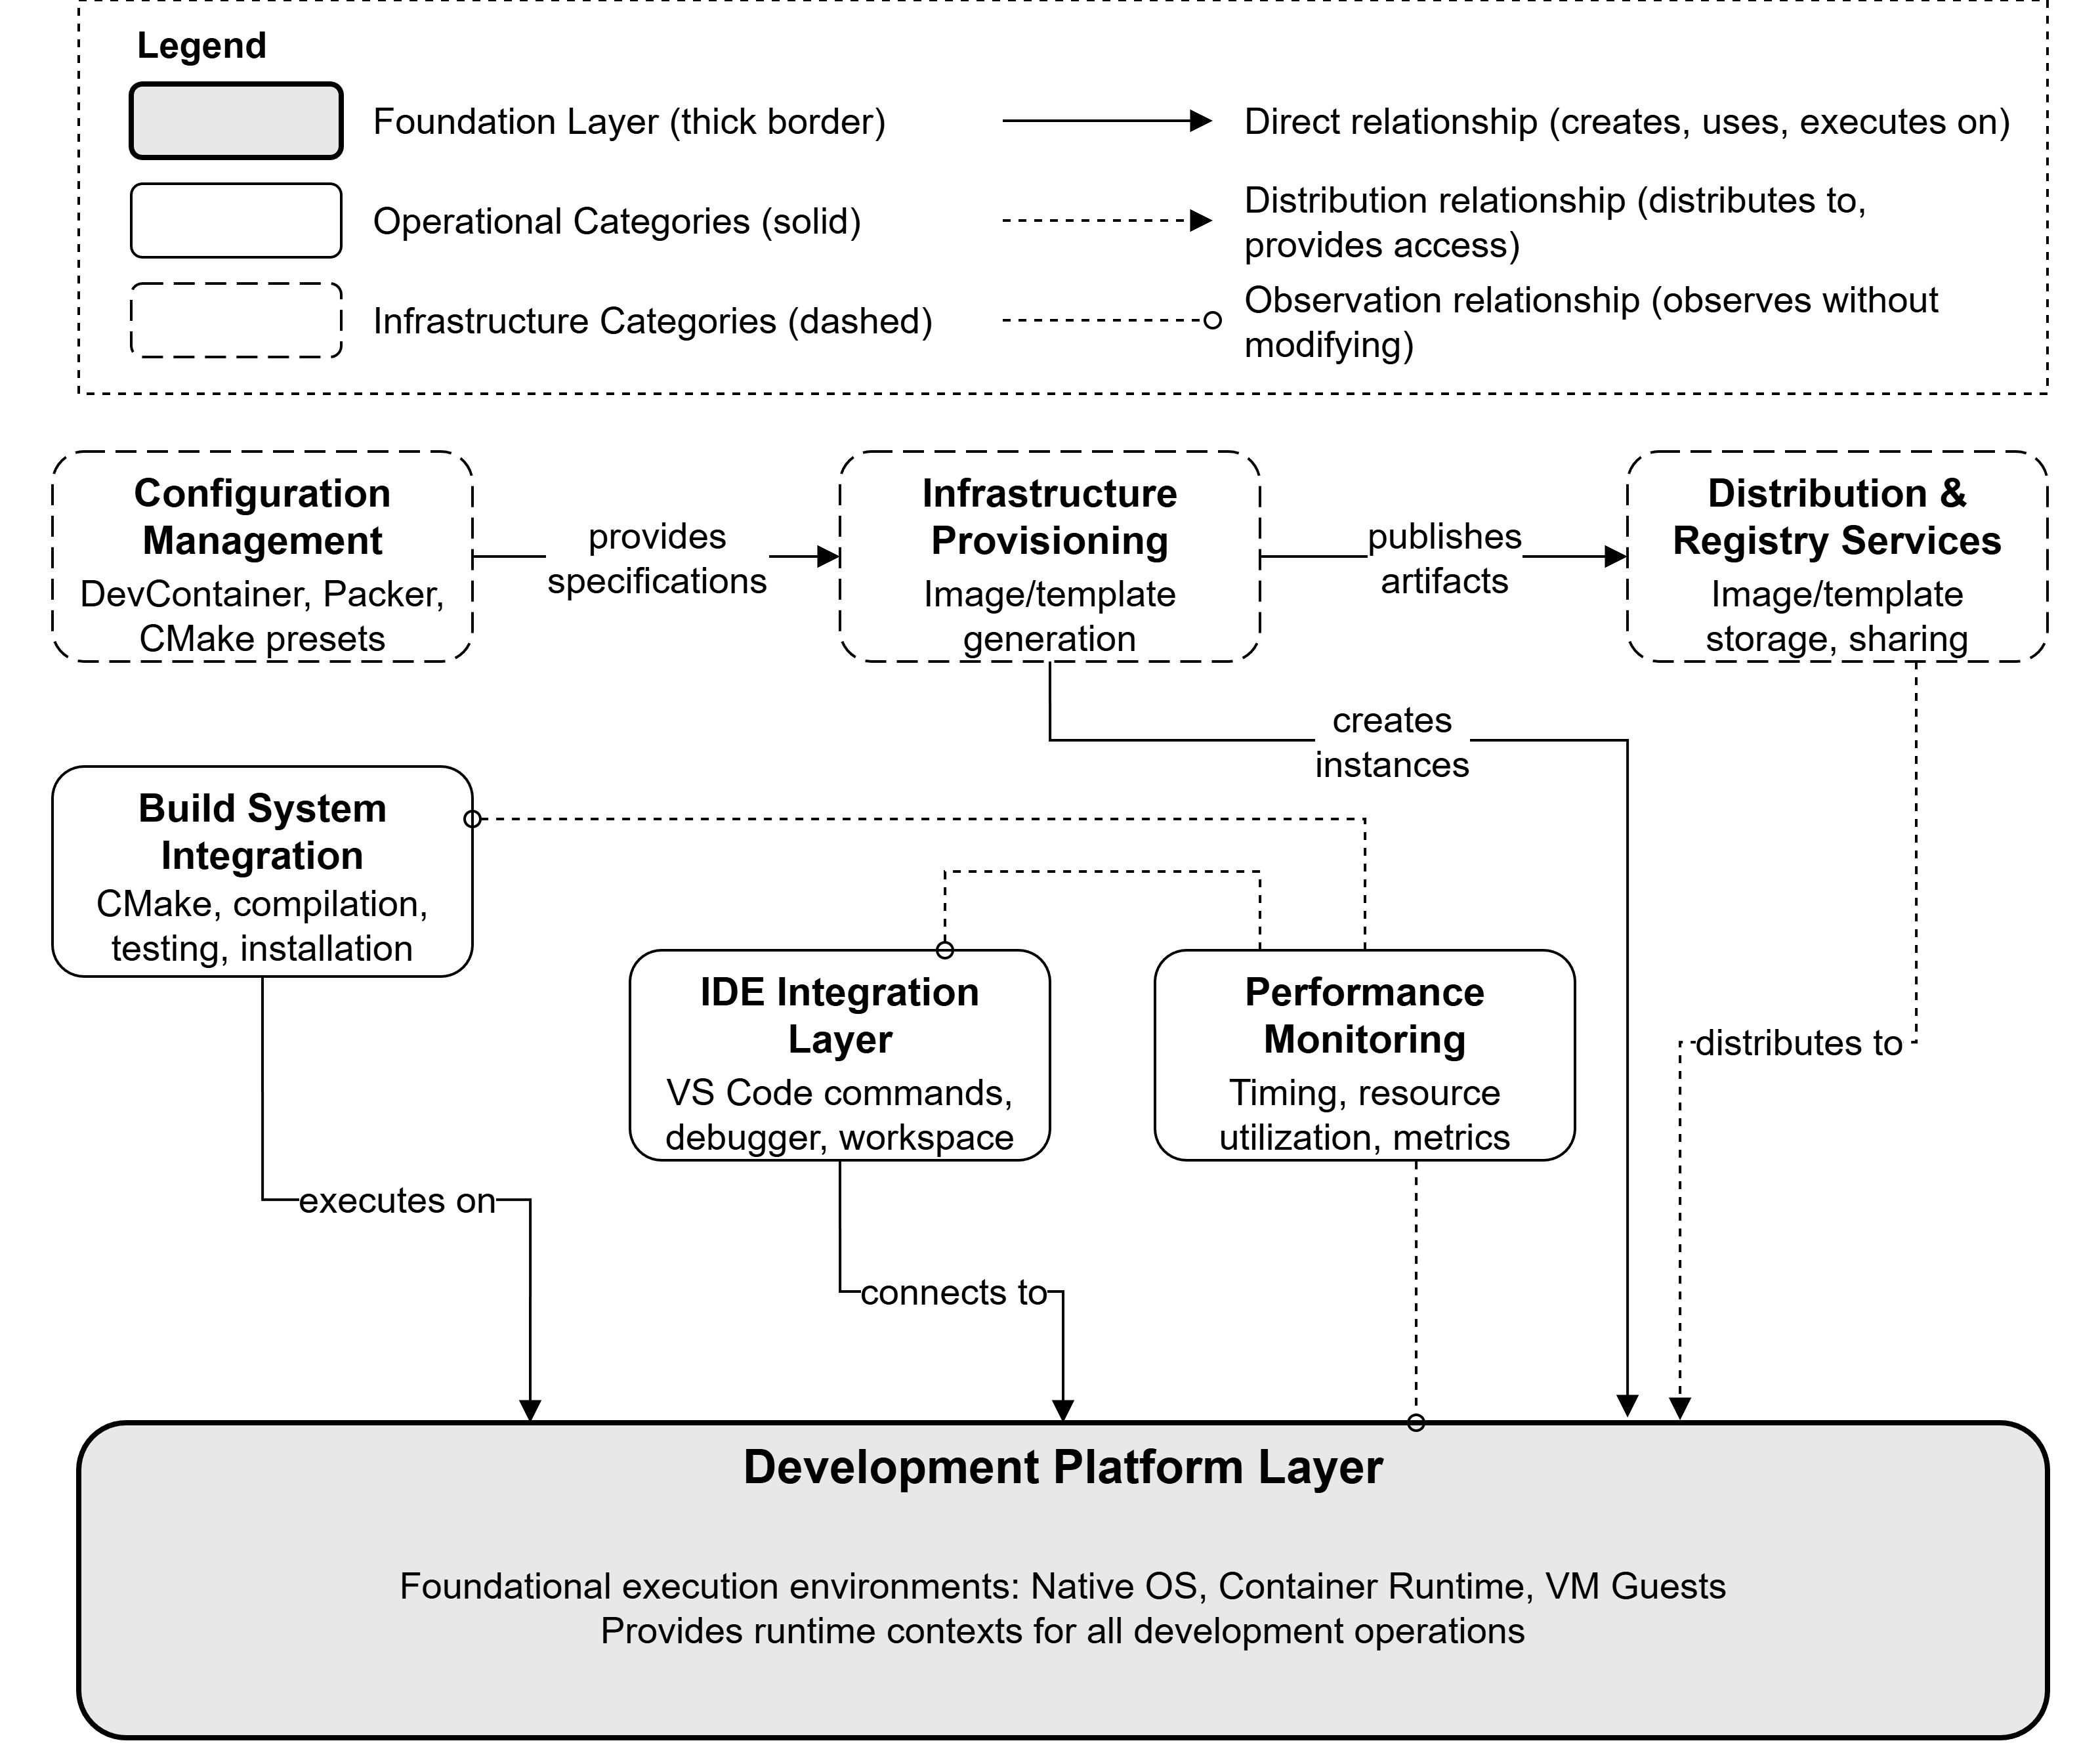
\includegraphics[width=0.90\linewidth]{figures/component-architecture-logical-view.png}
	\caption{Component Architecture - Logical View}
	\label{fig:logical-components}
\end{figure}
% [FIGURE: Diagram showing 7 component boxes with labeled associations between them. Components: Development Platform Layer (foundation), Build System Integration, Infrastructure Provisioning, Distribution & Registry Services, IDE Integration Layer, Performance Monitoring, Configuration Management. Show key relationships: Configuration Management provides specifications to Infrastructure Provisioning; Infrastructure Provisioning produces artifacts consumed by Distribution & Registry Services; Build System Integration executes on Development Platform Layer; IDE Integration Layer coordinates with Development Platform Layer; Performance Monitoring observes all categories; all operational components build upon Development Platform Layer as foundation.]

\subsubsection{Development Platform Layer Component}

The Development Platform Layer component describes the foundational execution environments that provide the runtime contexts for all development operations.
This component represents the three platform approaches being evaluated: native host operating systems, container runtimes, and virtual machine guests.
Rather than managing these platforms, the prototype leverages their distinct characteristics to enable comparative performance analysis.

This component serves as the foundational layer for comparative evaluation.
The three platform types provide distinct execution environments with measurable performance implications for day-to-day development workflows, making platform selection a critical architectural decision in legacy software development modernization.

\subsubsection{Build System Integration Component}

The Build System Integration component encapsulates all abstractions related to compilation, linking, testing, and installation workflows that execute within development environments.

This component provides the primary evaluation workload for measuring workflows across environment types, as build operations constitute frequent and resource-intensive development activities.

\subsubsection{Infrastructure Provisioning Component}

The Infrastructure Provisioning component encompasses mechanisms for creating deployment-ready development environments from declarative specifications.
For containerized environments, this includes automated image building from Dockerfiles.
For virtualized environments, this component focuses on VM instantiation from pre-existing templates.

This component represents the foundation infrastructure enabling reproducible environments, though provisioning occurs infrequently compared to daily build/test operations.

\subsubsection{Distribution \& Registry Services Component}

The Distribution \& Registry Services component manages environment definition sharing across development teams through centralized or distributed storage mechanisms.

This component enables evaluation scenarios where centralized infrastructure supports multiple developers, removing local environment build overhead from environment activation workflows.

\subsubsection{IDE Integration Layer Component}

The IDE Integration Layer component provides seamless connection between Visual Studio Code and underlying development environments regardless of environment type.

This component ensures developers interact with different environment types through identical interfaces, enabling fair productivity comparisons that isolate infrastructure differences from workflow differences.

\subsubsection{Performance Monitoring Component}

The Performance Monitoring component captures quantitative metrics enabling systematic evaluation of infrastructure approaches.

This component provides the empirical foundation for answering research questions regarding containerization impact on developer productivity.

\subsubsection{Configuration Management Component}

The Configuration Management component defines declarative specifications governing environment behavior and build parameters.

This component provides the declarative foundation enabling reproducible environments that developers can modify, version, and share as code artifacts.

\subsubsection{Component Relationships}

The architectural components interact through well-defined relationships that establish information flow and responsibility boundaries:

\begin{itemize}
\item \textbf{Development Platform Layer $\rightarrow$ All Operational Components:} Foundation relationship where the platform layer provides execution contexts for all operational components (builds execute on platforms, IDE connects to platforms, monitoring observes platform behavior)
\item \textbf{Configuration Management $\rightarrow$ Infrastructure Provisioning:} Configuration specifications (DevContainer configurations, VM deployment scripts, CMake presets) define environment characteristics consumed by provisioning workflows
\item \textbf{Infrastructure Provisioning $\rightarrow$ Distribution \& Registry Services:} Provisioned artifacts (container images, VM templates) are published to registries and repositories for team distribution
\item \textbf{Infrastructure Provisioning $\rightarrow$ Development Platform Layer:} Provisioning creates the platform instances (VMs, container images, native toolchain installations) that constitute the Development Platform Layer
\item \textbf{Distribution \& Registry Services $\rightarrow$ Development Platform Layer:} Distributed artifacts enable instantiation of new platform instances from centralized sources
\item \textbf{Build System Integration $\rightarrow$ Development Platform Layer:} Build operations execute within platform contexts, consuming platform-provided resources (compilers, CPU, filesystem)
\item \textbf{IDE Integration Layer $\rightarrow$ Development Platform Layer:} IDE connects to platforms through platform-specific protocols (native process spawning, Docker API, SSH to VMs) and coordinates workspace access
\item \textbf{Performance Monitoring $\rightarrow$ All Components:} Observation relationship where monitoring instruments operations across all components without modifying their behavior
\end{itemize}

This component-based architecture provides a high-level logical organization suitable for describing system functionality without prescribing specific implementation approaches.
The abstraction level enables flexible implementation choices while maintaining clear responsibility boundaries and relationships between major functional areas.
The architecture supports the evaluation framework by clearly separating the foundational platforms being evaluated (Development Platform Layer) from the operational components that execute identically across platforms (Build System Integration, Configuration Management), enabling systematic comparison of platform approaches while holding other variables constant.

\subsection{Interface Design}

The prototype distinguishes between development interfaces and infrastructure provisioning interfaces, each optimized for their respective usage frequency and audience.

\subsubsection{Development Interface}

The primary development interface combines VS Code's DevContainer extension with CMake Tools, enabling developers to work within containerized or virtualized environments using familiar IDE interactions \citep{microsoftDevelopingContainer2025, swidzinskiModernCMakeEffortlessly2024}.

In case of containers, environment activation occurs through a single command (``Reopen in Container''), which provisions the development environment, installs extensions, and establishes workspace connectivity.
Once activated, developers interact with the environment identically to native development: selecting CMake presets through status bar dropdowns, triggering builds with keyboard shortcuts, and viewing test results in integrated panels.
The interface abstracts the environment type entirely, ensuring identical workflows whether compilation occurs directly on a (virtual) machine or in a container.

\subsubsection{Infrastructure Interface}

Infrastructure provisioning uses direct command-line tools and simple helper scripts rather than elaborate interface abstractions.
Container images are built with \texttt{docker build} and distributed with \texttt{docker push}.
VM instantiation uses platform-native tools (PowerShell cmdlets and Hyper-V Manager for Hyper-V on Windows 11).
Pre-existing VM templates are assumed to be available from local storage or network shares.

\newpage
\section{Development View}

The Development View describes the static organization of the software artifacts in the development environment, focusing on how code, configuration files, scripts, and other development artifacts are structured, managed, and maintained.
This view addresses concerns of developers and project managers regarding modular organization, code reuse, compilation dependencies, and release management \citep{kruchten4+1ViewModel1995}.

\subsection{Code and Artifact Organization}

The prototype software is organized into a layered hierarchy, separating concerns between infrastructure automation, environment definitions, build configurations, and IDE integration.
This layered architecture enables independent development and maintenance of different system aspects while ensuring clear dependency relationships and promoting reusability.

\subsubsection{Layer 1: Infrastructure Automation Scripts}

The foundation layer contains infrastructure-as-code artifacts that automate development environment deployment.

\textbf{VM Template Repository:} Pre-existing VM templates for Hyper-V as target platform, covering Windows Server and Debian Linux as target operating systems with semantic versioning enabling parallel maintenance of multiple toolchain generations.

\textbf{Deployment Automation Scripts:} Platform-specific VM instantiation scripts using PowerShell cmdlets and Hyper-V Manager that clone templates from local storage or network shares, apply configurations, and initialize VMs for development use.

\subsubsection{Layer 2: Environment Definition Artifacts}

The second layer contains declarative environment specifications that define development environment requirements independent of specific infrastructure implementations.

\textbf{Dockerfile Definitions:} Multi-stage Dockerfile definitions organized by Linux distribution (Debian Linux, AlmaLinux) and version.
Dockerfiles follow consistent structure: base image selection, system package installation, development tool installation, environment configuration, and user setup.
Layer ordering optimizes build cache utilization, placing infrequently-changing dependencies in early stages.

\textbf{DevContainer Specifications:} JSON-format DevContainer definitions (.devcontainer/devcontainer.json) that declare container-based development environments.
Specifications reference Dockerfiles or pre-built images and define VS Code extensions, workspace mounts and port forwards.

\subsubsection{Layer 3: Build System Configuration}

The third layer encapsulates build system configurations that standardize compilation across different development environments.

\textbf{CMake Preset Files:} JSON-format preset definitions (CMakePresets.json) organizing build configurations through inheritance hierarchies.
Base presets define common parameters, platform-specific presets add compiler selection and flags, and build-type presets specify optimization levels.

\textbf{CMake Project Configuration:} The CMakeLists.txt hierarchy defining the complete build system: target management, tool availability checks, third-party dependency inclusion, CTest integration, and installation rules.
Generator expressions and conditional logic enable support for multiple compilers (MSVC, GCC, Clang).

\subsubsection{Layer 4: IDE Integration Artifacts}

The fourth layer provides integration between development environments and Visual Studio Code, abstracting complexity through IDE-native mechanisms.

\textbf{VS Code Task Definitions:} JSON-format task configurations (.vscode/tasks.json) defining test, and deployment operations.
Tasks integrate with CMake presets through variable substitution, enabling GUI-based workflow invocation.

\textbf{VS Code Launch Configurations:} Debugger attachment configurations (.vscode/launch.json) supporting both native and remote debugging scenarios.
Launch configurations adapt to environment type (native, container, VM), automatically adjusting debugger paths and symbol resolution.

\textbf{VS Code Extension Configurations:} Settings files (.vscode/settings.json, .vscode/extensions.json) defining required extensions and workspace-specific configurations.

\subsubsection{Layer 5: Documentation}

The top layer contains documentation and developer guidance.

\textbf{Documentation} Markdown-format documentation organized by topic (setup guides, architecture descriptions, contribution guidelines).
Documentation artifacts version alongside code, ensuring consistency between implementation and descriptions.

\subsubsection{Dependency Management and Build Order}

The layered organization enforces clear compilation dependencies and enables independent development:
% TODO : Add diagram showing layers and dependencies? or delete this section
\begin{itemize}
\item \textbf{Layer 1 independence:} Infrastructure scripts have no dependencies on higher layers, enabling infrastructure changes without affecting build configurations or IDE integration
\item \textbf{Layer 2 to Layer 1:} Environment definitions depend on infrastructure scripts only for template-based VM configurations; container definitions are fully independent
\item \textbf{Layer 3 to Layer 2:} Build configurations reference environment capabilities (compilers, tools) but remain environment-agnostic through preset abstraction
\item \textbf{Layer 4 to Layers 2-3:} IDE integration depends on environment definitions (DevContainer specs) and build configurations (CMake presets) but adds no new functional requirements
\item \textbf{Layer 5 to all:} Documentation references all layers but has no compilation dependencies
\end{itemize}

This dependency structure supports incremental development, enabling modifications to infrastructure automation without impacting build system configurations, or changes to IDE integration without affecting core build definitions.

\subsection{Technology Stack and Implementation}

The prototype leverages a carefully selected technology stack that balances functionality, performance, and maintainability requirements while enabling comprehensive comparison between virtualization and containerization approaches.

\subsubsection{Infrastructure Automation Technologies}

Hyper-V serves as the virtualization platform for VM-based development environment evaluation on Windows 11 hosts.
Initial testing revealed compatibility issues with VirtualBox, including the inability to run with hardware acceleration on Windows 11 hosts and compatibility problems on Debian 12 hosts.
Consequently, all virtualization tests were conducted using Hyper-V on Windows 11 hosts.
VM templates are imported via PowerShell cmdlets and Hyper-V Manager, enabling scripted deployment from VHDX images stored locally or on network shares.

\subsubsection{Containerization Technologies}

Docker Engine provides the core containerization platform with BuildKit support for advanced build features \citep{dockerDockerReferenceDocumentation2025}.
Multi-stage builds, layer caching, and build-time secrets enable efficient, secure container image generation.
The Docker CLI provides command-line interfaces for image building, container management, and registry operations.

The DevContainer specification standardizes development environment definitions for VS Code integration \citep{DevelopmentContainers2025}.
Feature specifications enable modular tool installation without custom Dockerfile creation, while lifecycle hooks provide initialization and cleanup capabilities.
Listing \ref{lst:devcontainer-example} demonstrates a DevContainer configuration structure.

\newpage
\begin{lstlisting}[caption={DevContainer Configuration Structure},label=lst:devcontainer-example]
{
  "name": "C++ Development Container - Debian 12",
  "image": "debian:bookworm",
  "features": {
    "ghcr.io/devcontainers/features/cmake:1": {},
    "ghcr.io/devcontainers/features/ninja-build:1": {}
  },
  "customizations": {
    "vscode": {
      "extensions": [
        "ms-vscode.cpptools",
        "ms-vscode.cmake-tools"
      ]
    }
  }
}
\end{lstlisting}

\subsubsection{Build System Integration}

CMake provides cross-platform build system generation with comprehensive preset support \citep{swidzinskiModernCMakeEffortlessly2024}.
The preset system enables declarative build configuration with support for inheritance, environment variable expansion, and conditional preset selection based on host platform characteristics.
The preset hierarchy establishes three levels: base presets defining common parameters shared across all configurations, platform-specific presets inheriting from base presets while adding compiler flags and toolchain specifications, and specialized build-type presets (Debug, Release, RelWithDebInfo) that further refine optimization settings.
Listing \ref{lst:cmake-preset-example} illustrates the structure of a CMake preset configuration.

\begin{lstlisting}[caption={CMake Preset Configuration Structure},label=lst:cmake-preset-example]
{
  "configurePresets": [
    {
      "name": "base",
      "hidden": true,
      "generator": "Ninja",
      "cacheVariables": {
        "CMAKE_EXPORT_COMPILE_COMMANDS": "ON"
      }
    },
    {
      "name": "linux-base",
      "inherits": "base",
      "condition": {
        "type": "equals",
        "lhs": "${hostSystemName}",
        "rhs": "Linux"
      },
      "cacheVariables": {
        "CMAKE_C_COMPILER": "gcc",
        "CMAKE_CXX_COMPILER": "g++"
      }
    }
  ]
}
\end{lstlisting}

CTest (integrated with CMake) enables automated test execution with parallel execution, timeout management, result reporting, and integrates with VS Code through the CMake Tools extension for test discovery and visualization.

Ninja serves as the build backend, providing faster build execution than traditional Make through parallel compilation and intelligent dependency tracking.

\subsubsection{Development Environment Integration}

Visual Studio Code provides the integrated development environment with C++ development support \citep{microsoftDevelopingContainer2025}.
The C/C++ extension (ms-vscode.cpptools) provides IntelliSense, debugging, and code navigation capabilities.
The CMake Tools extension (ms-vscode.cmake-tools) integrates CMake configuration, building, and testing within the IDE.
The Remote - Containers extension (ms-vscode-remote.remote-containers) enables development within Docker containers with full IDE feature support.

\subsubsection{Version Control and CI/CD Integration}

Git provides distributed version control for source code, infrastructure definitions, and environment configurations using the git-flow branching model with feature, release, and hotfix branches \citep{driessenSuccessfulGitBranching2010}.

Optional CI/CD integration can leverage local build servers or cloud-based platforms for automated builds, tests, and deployments, though the primary evaluation focuses on local development workflows and workstation performance.

\subsection{Build and Deployment Processes}

The prototype implements automated build and deployment processes, figure \ref{fig:build-deployment-pipeline} illustrates the overall workflow.

\begin{figure}[ht!]
	\centering
	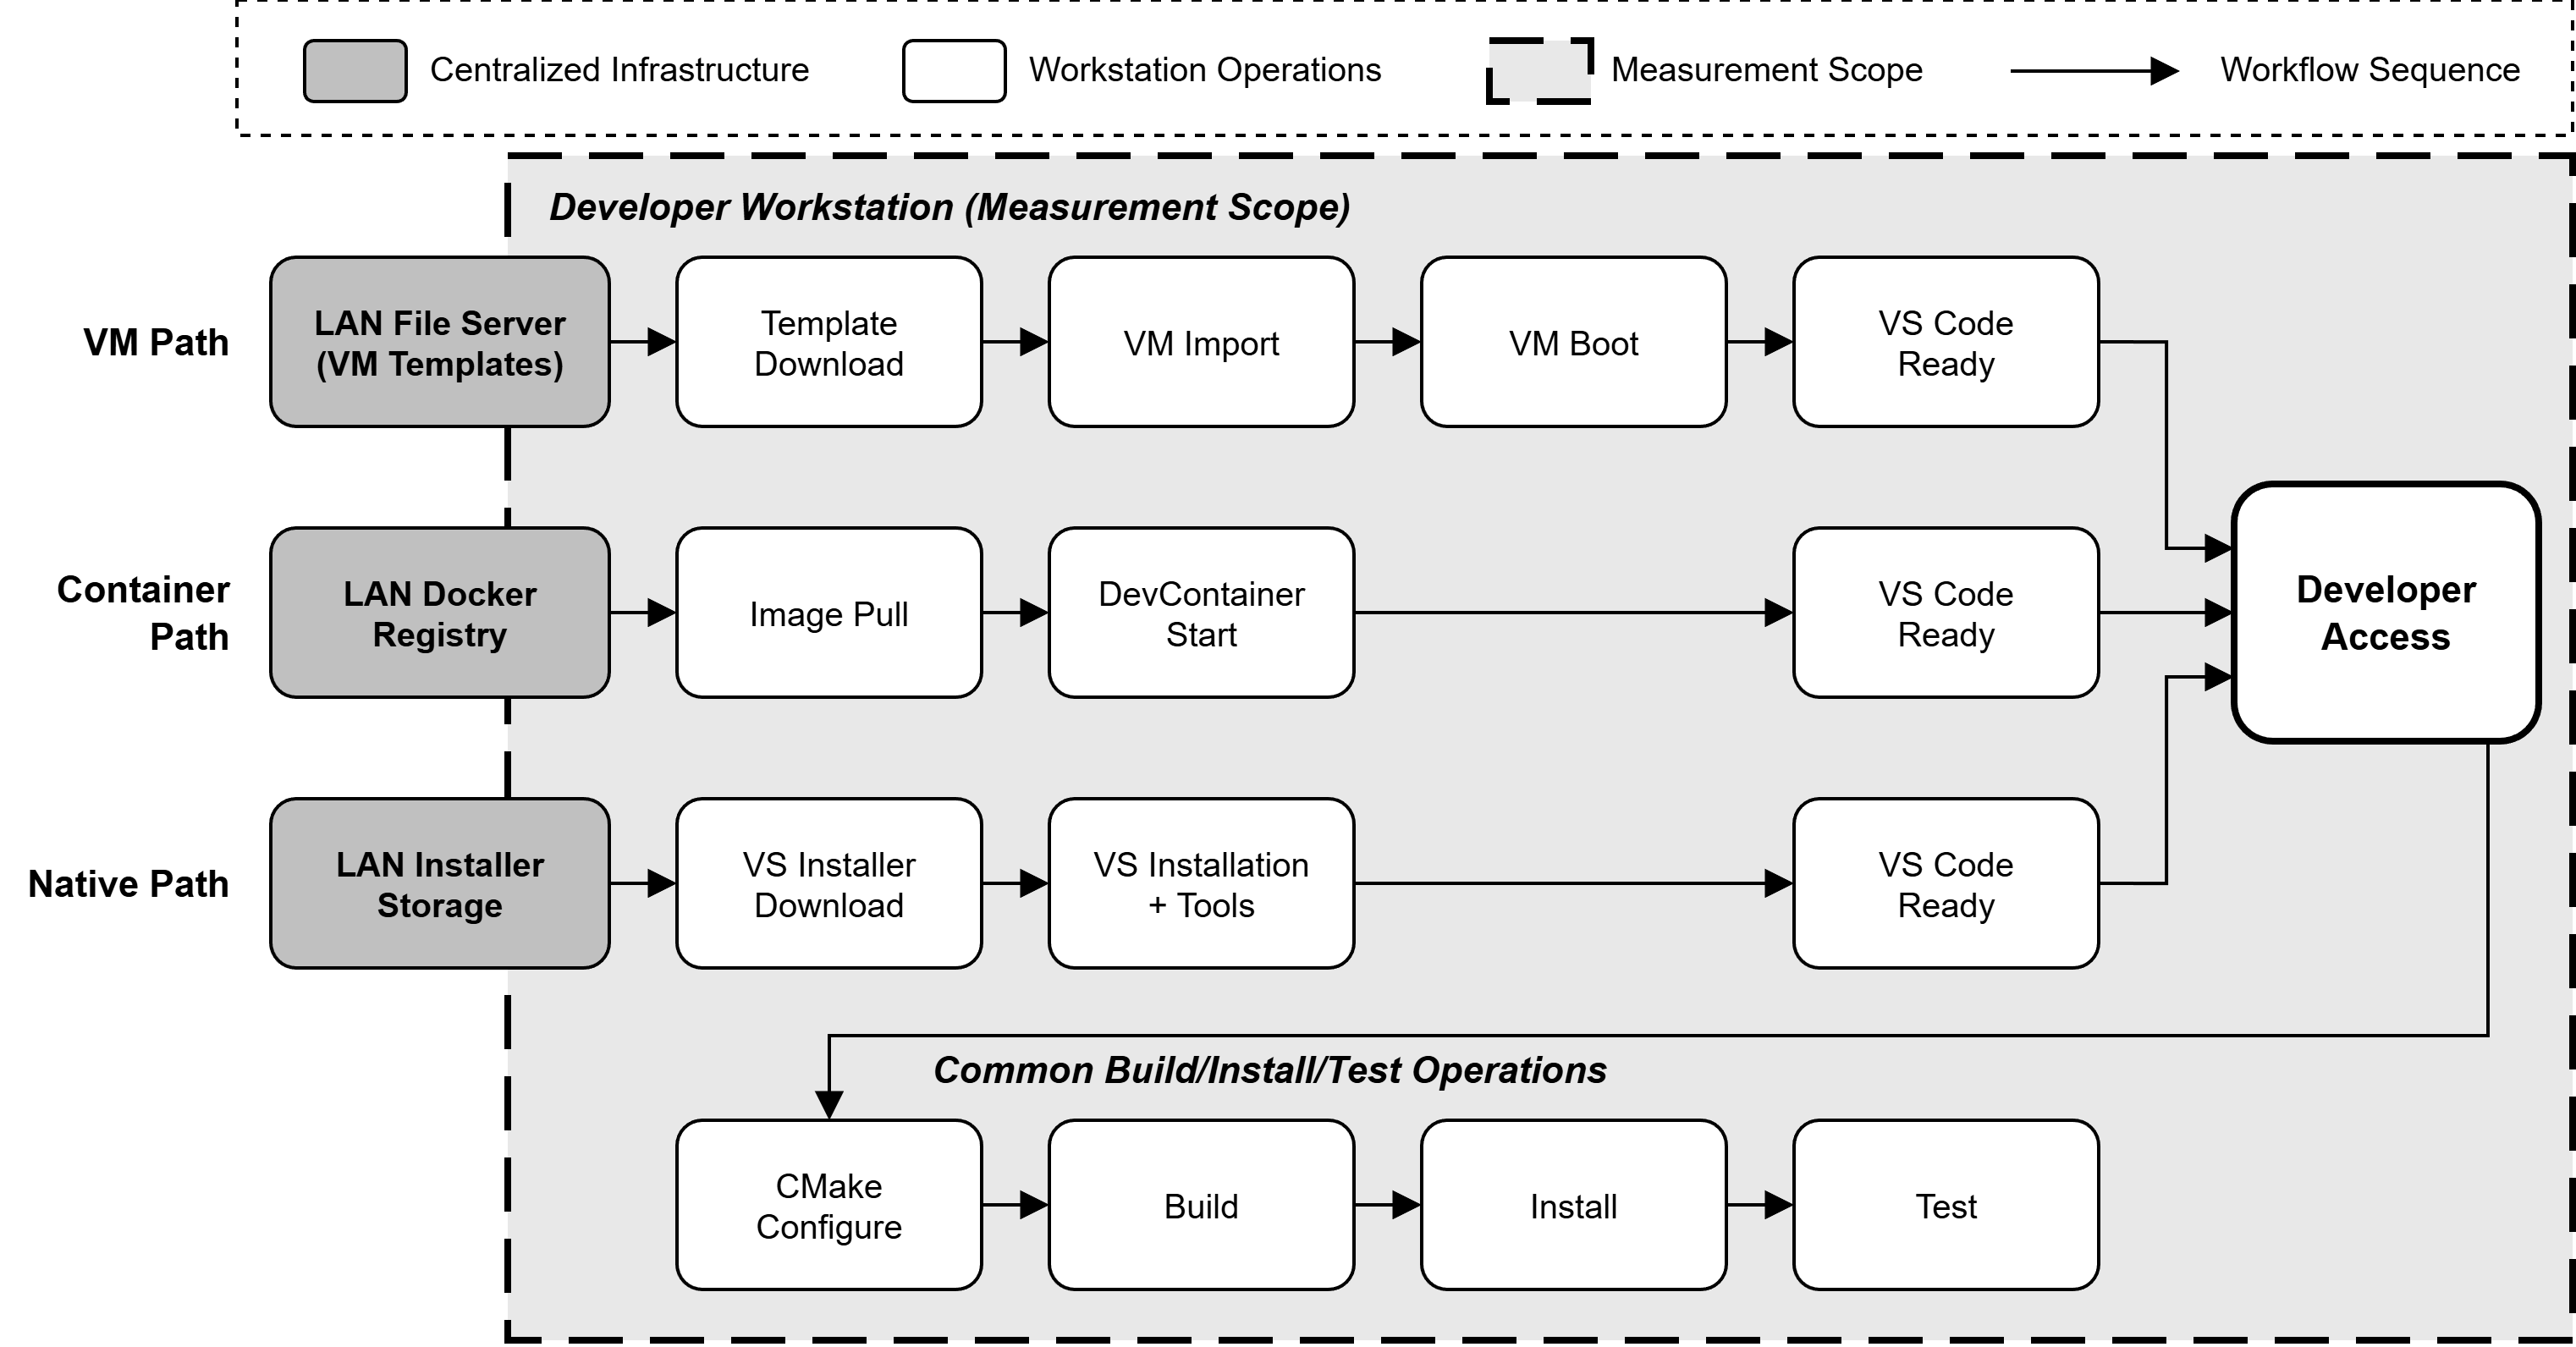
\includegraphics[width=\linewidth]{figures/build-deployment-pipeline.png}
	\caption{Build and Deployment Processes}
	\label{fig:build-deployment-pipeline}
\end{figure}
% [FIGURE: Flow diagram showing three parallel environment provisioning paths converging at developer access: 1) VM Path: LAN File Server (VM Templates) → VBoxManage Import → VM Boot → Developer Access, 2) Container Path: LAN Docker Registry → Image Pull → DevContainer Start → Developer Access, 3) Native Path: LAN Installer Storage → Visual Studio Installation → Developer Access. Emphasizes that all artifact sources are pre-built and centrally distributed, with deployment to developer workstation as the measured scope.]

\newpage
\subsubsection{Environment Provisioning and Deployment}

VM template generation and container image generation occur centrally within organizational infrastructure rather than on developer workstations, producing artifacts distributed from central infrastructure (LAN file shares for VM templates, container registries for Docker images).
The evaluation focuses on activation/deployment time and day-to-day development operations, measuring only the time to activate a development environment from pre-existing artifacts.

\textbf{Hyper-V VM Deployment:} PowerShell scripts and Hyper-V Manager automate deployment by importing VHDX template files from local or network storage, applying VM-specific parameters (hostname, memory allocation, CPU core count), configuring network attachment to virtual switches, and initiating VM startup.
All virtualization testing was conducted using Hyper-V on Windows 11 hosts after initial tests revealed VirtualBox compatibility issues with hardware acceleration on Windows 11 and stability problems on Debian 12 hosts.
Measurements capture: local template instantiation duration (VM creation and initial boot); LAN template download duration (20GB, dependent on network bandwidth); VM configuration time; first boot and initialization duration; total time from deployment initiation to functional development environment.

\textbf{Docker Container Deployment:} DevContainer activation workflow automates environment setup by pulling container image layers from registry (with local cache reuse when image exists locally), creating containers from pulled images with configured volume mounts and network settings, installing VS Code server and extensions within the container, and executing post-creation initialization scripts.
Measurements capture: image pull duration from LAN registry (2GB compressed layers, dependent on network bandwidth); container creation and startup time; VS Code server and extension installation duration; post-creation script execution time; total time from activation initiation to functional development environment.

\textbf{Native Environment Setup:} Native deployment downloads Visual Studio installer from LAN infrastructure (approximately 10GB) followed by manual installation and configuration procedures.
Measurements capture: Visual Studio installer download (via LAN) and installation duration.
Task switching scenarios requiring different Visual Studio versions may necessitate complete uninstallation and reinstallation, as discussed in the scenario evaluation section.

\textbf{Comparative Characteristics:} All three approaches require comparable initial network bandwidth for artifact distribution (VMs: 20GB templates; containers: 2GB compressed images; native: 10GB VS installer).
VM deployment requires a full additional OS to boot and to manage and provides persistent long-lived environments with continuous resource consumption even when idle.
Container deployment completes startup in seconds and enables flexible resource management by stopping containers when not in use and restarting rapidly when needed.
Native deployment requires manual configuration introducing human error risk and configuration drift over time, with potential reinstallation overhead during environment switching.

\section{Process Architecture}

The Process View addresses the runtime and concurrency aspects of the prototype system, describing the processes and resource contention that occur during development operations across native, virtualized, and containerized environments \citep{kruchten4+1ViewModel1995}.

\subsection{Runtime Process Decomposition}

The prototype system executes through multiple concurrent processes distributed across host systems, virtual machines, and containers.
Understanding this process architecture enables analysis of performance bottlenecks and resource contention patterns.

\subsubsection{Native Development Process Architecture}

In native development environments, all processes execute directly on the host operating system.

The \textbf{IDE process} provides the development interface and spawns child processes for build system operations.
The \textbf{CMake configuration process} executes during initial setup and parameter changes, detecting compilers and generating build files.
The \textbf{Ninja build process} coordinates parallel compilation by spawning multiple compiler processes (MSVC cl.exe on Windows, gcc/g++ on Linux) matching CPU core count.
The \textbf{CTest execution process} manages parallel test execution, spawning test executable processes concurrently.

All processes access host resources directly without virtualization overhead, but may experience resource contention when parallel operations exceed available CPU cores or memory.

\subsubsection{Virtualized Development Process Architecture}

Virtualized development introduces hypervisor-managed process layers.

The \textbf{hypervisor host service} (Hyper-V Virtual Machine Management Service on Windows 11) manages VM lifecycle and allocates resources to guest VMs.
Within the \textbf{guest VM}, the complete native process architecture executes but operates on virtualized hardware.
With all logical cores assigned to the guest VM, processes have direct access to CPU resources with minimal hypervisor scheduling overhead, though virtualization overhead from hardware abstraction remains.

Guest-level parallelism benefits from the full CPU allocation strategy, eliminating artificial resource constraints while maintaining hypervisor-level virtualization overhead.
VM management operations (provisioning, snapshot) consume significant CPU and I/O resources.

\subsubsection{Containerized Development Process Architecture}

Containerized development leverages Linux container isolation with distinct characteristics.

The \textbf{Docker daemon} (dockerd) manages container lifecycle on the host (or within WSL2 on Windows).
Within containers, development processes execute in isolated namespaces: IDE server, CMake, Ninja, compilers, and test executables.
Container processes access host CPU directly without virtualization overhead, though cgroup resource limits may apply.

Filesystem access patterns depend on mount strategy: bind mounts traverse multiple layers (container namespace → Docker filesystem → host filesystem), while named volumes provide optimized Docker-managed storage.
On Windows, bind mount operations experience higher overhead due to WSL2 filesystem translation.

\subsection{Parallelism and Resource Contention}

The build and test processes achieve parallelism through Ninja's and CTest's multi-process coordination.
Ninja spawns compiler workers up to the configured parallelism limit (typically matching CPU cores), while CTest spawns test processes similarly.

Resource contention manifests differently across environments:
\textbf{Native environments} experience direct CPU, memory, and I/O contention when parallel processes exceed available resources.
\textbf{Virtualized environments} with all logical cores assigned minimize hypervisor CPU scheduling contention but retain virtualization overhead from hardware abstraction layers.
\textbf{Containerized environments} on Windows with bind mounts amplify filesystem I/O contention through layered filesystem operations.

IDE communication varies by environment: native and virtualized development uses direct process spawning and containerized development uses Docker APIs with lower overhead than VM-based approaches.

\subsection{Performance Monitoring}

The prototype employs a Python-based cross-platform benchmark monitor for capturing performance metrics during development operations.

The monitoring solution utilizes the \textbf{psutil library} providing unified access to system resources across Windows and Linux through a consistent API abstracting platform-specific implementations.

The benchmark monitor captures system-wide metrics rather than per-process measurements due to the highly parallel nature of build and test operations:
\begin{itemize}
\item \textbf{Timing measurements}: Wall-clock duration for discrete operations using Python's time.perf\_counter()
\item \textbf{CPU metrics}: System-wide CPU utilization percentage across all cores
\item \textbf{Memory metrics}: System-wide memory consumption (total used, available, percentage)
\end{itemize}

Before each benchmark run, the monitor establishes a \textbf{baseline measurement} capturing idle system resource consumption to enable isolation of development operation overhead from background system activity.

For virtualized and containerized environments, monitoring adapts to specific characteristics: Windows VMs capture host-level memory usage of the VM process plus guest-internal metrics; Debian VMs rely solely on guest-internal monitoring; Docker Desktop on Windows tracks WSL2 VM memory consumption plus container-internal metrics.
CPU monitoring on the host is omitted for virtualized environments since all logical cores are assigned to guests.

The monitor operates as a lightweight background process consuming minimal resources (<1\% CPU) to minimize observer effects.
Metrics are logged to structured JSON files enabling post-processing, statistical analysis, and visualization of performance characteristics across development environments.

\section{Physical Architecture}

The Physical View describes the deployment topology and hardware infrastructure supporting the prototype evaluation environment.
This view provides essential context for understanding performance measurement conditions and ensures reproducible experimental results \citep{kruchten4+1ViewModel1995}.

\subsection{Test Environment Topology}

The prototype evaluation environment implements a controlled infrastructure setup designed to minimize external variables while supporting comprehensive performance measurement across native, virtualized, and containerized development approaches.
Figure \ref{fig:physical-architecture} illustrates the physical infrastructure topology.

\begin{figure}[ht!]
	\centering
	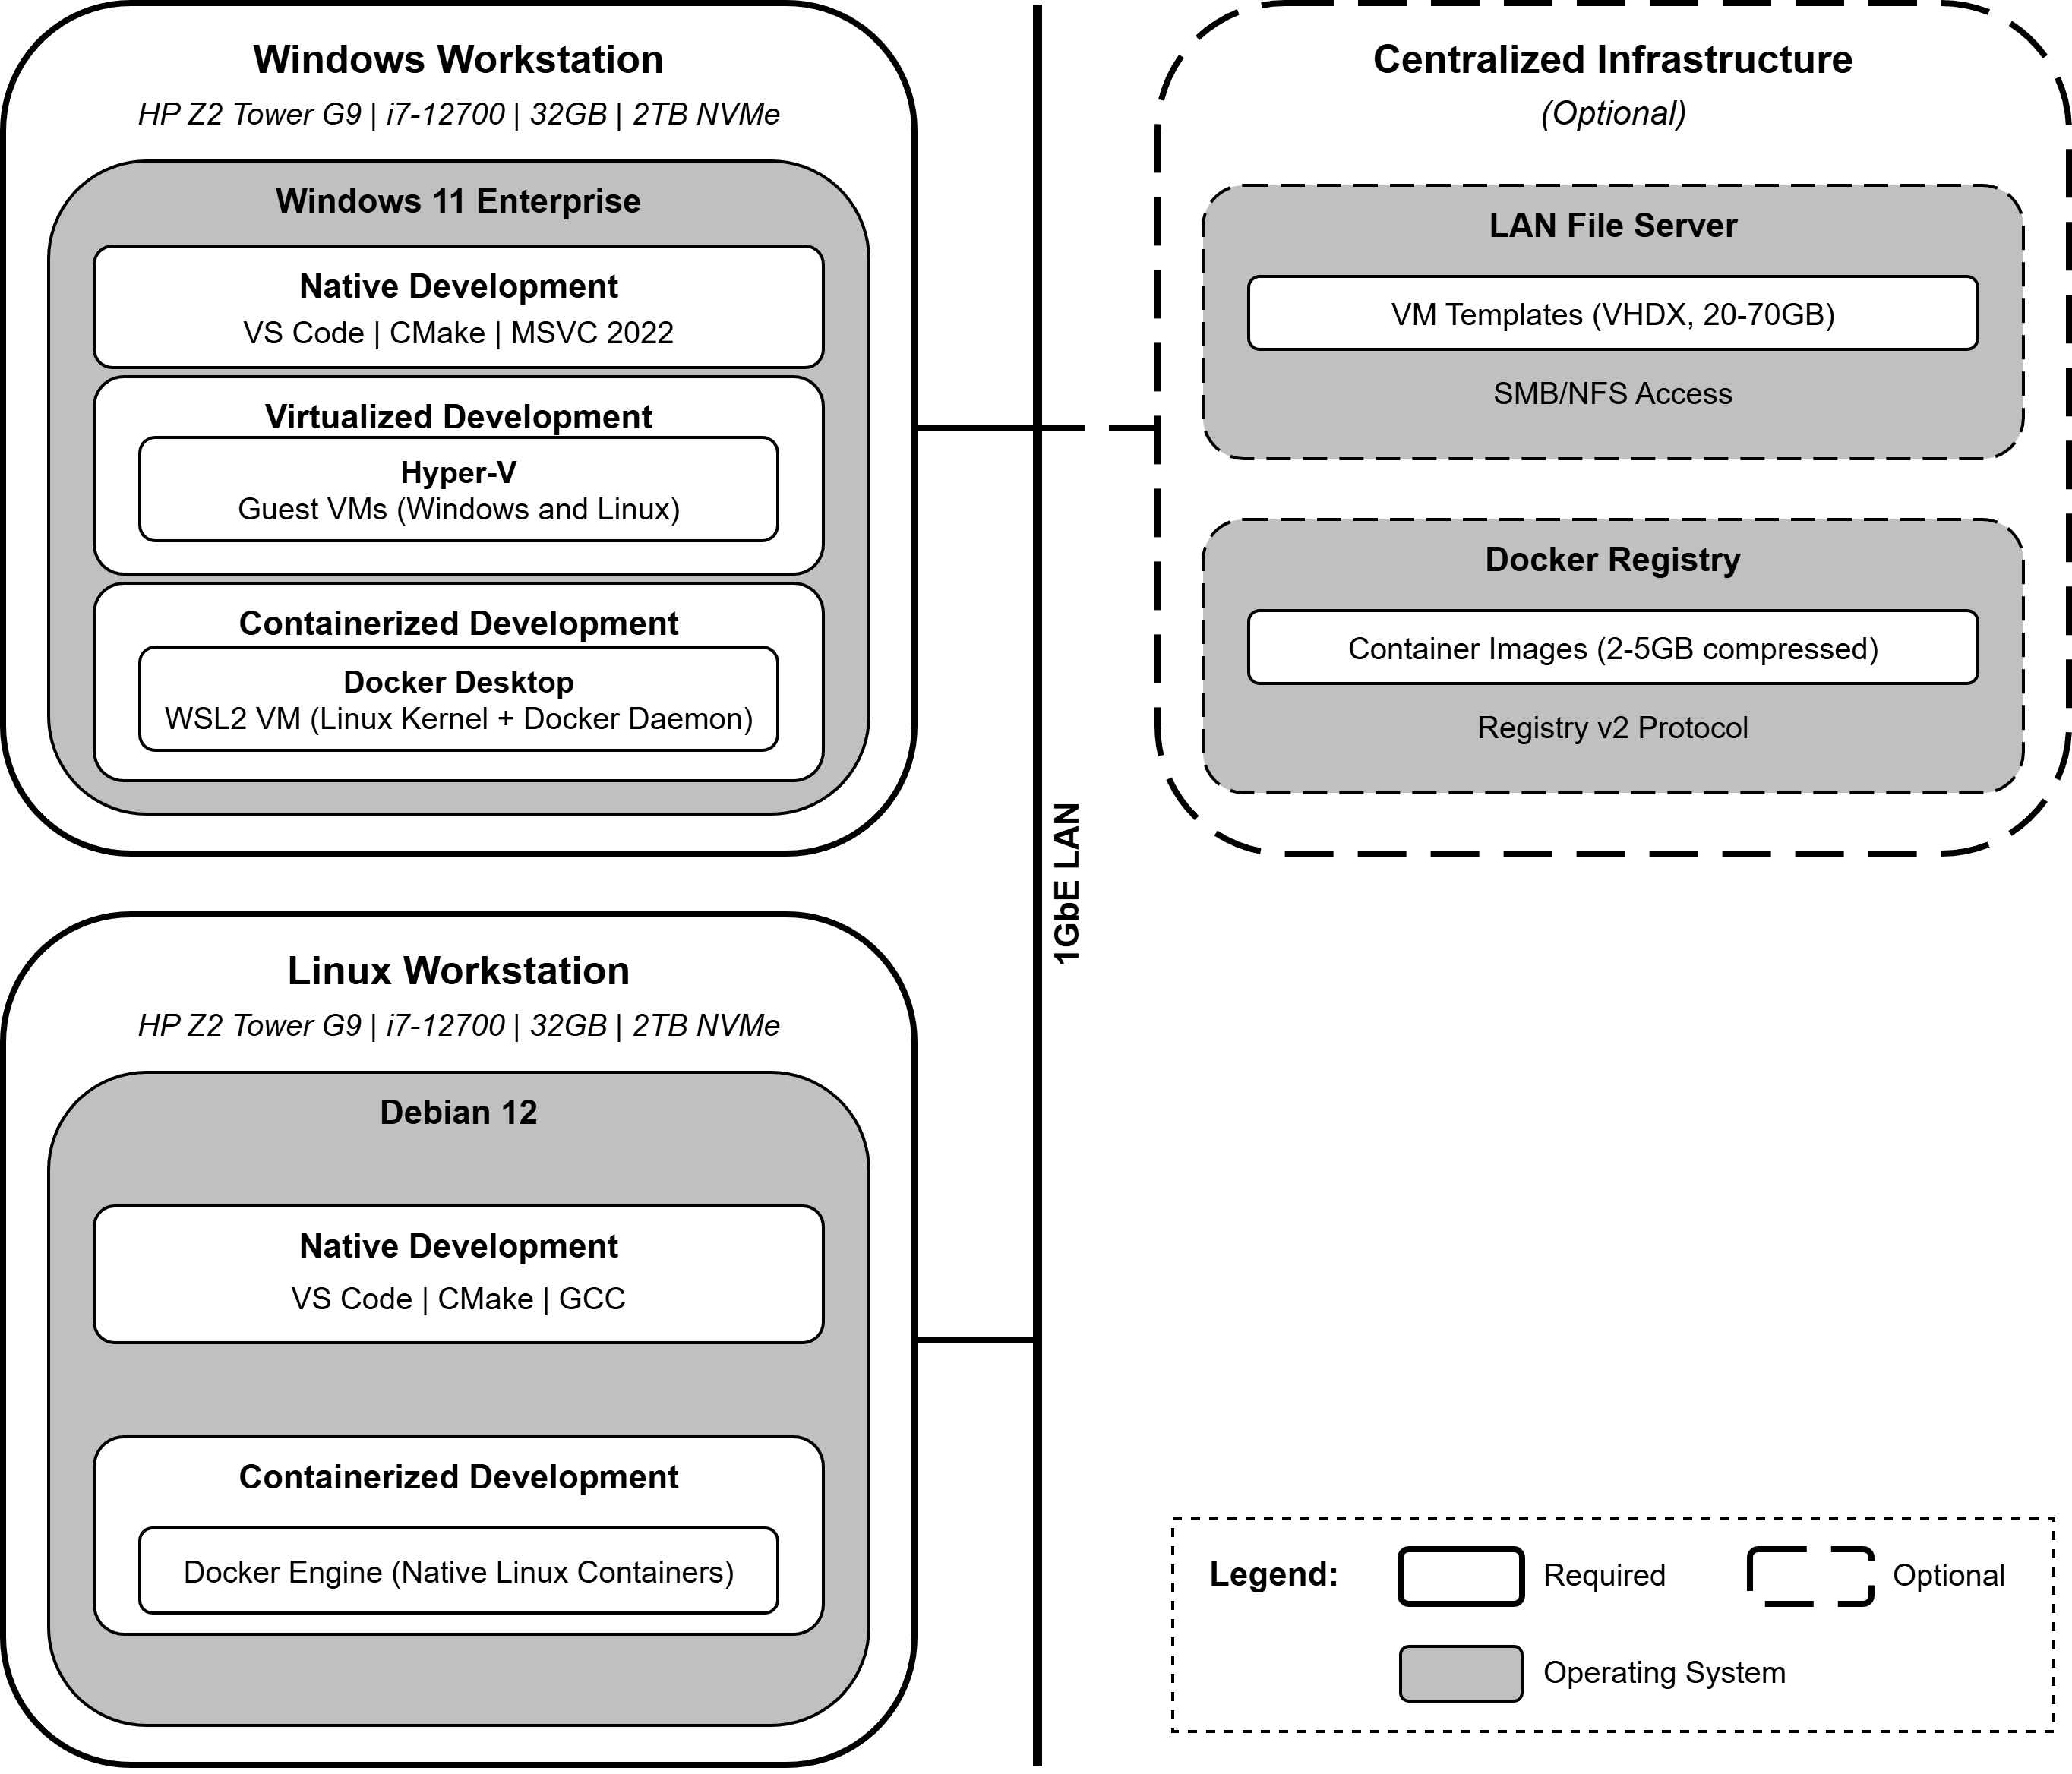
\includegraphics[width=0.90\linewidth]{figures/physical-architecture.png}
	\caption{Physical Architecture - Test Environment Topology}
	\label{fig:physical-architecture}
\end{figure}
% [FIGURE: Physical infrastructure topology showing: HP Z2 Tower G9 workstations supporting three deployment configurations (native, VM, container) on identical hardware. Windows workstations (Windows 11, Docker Desktop/WSL2) and Linux workstations (Debian 12, Docker Engine, VirtualBox) connected via 1GbE to optional centralized infrastructure: LAN file server (VM templates via SMB/NFS) and Docker registry (container images). Side-by-side comparison layout emphasizing controlled test environment with standardized hardware.]

\newpage
\subsubsection{Development Workstation Infrastructure}

The evaluation environment centers on standardized HP Z2 Tower G9 workstations that support native development, local virtualization, and containerization approaches on identical hardware.

All evaluation workstations use identical hardware: Intel Core i7-12700 processor (12 cores, 20 threads), 32GB DDR5-4800 RAM, 2TB PCIe 4.0 NVMe SSD, and 1GbE network connectivity.

Windows workstations run Windows 11 Enterprise LTSC 24H2 with Hyper-V enabled for both virtualization testing and Docker Desktop (with WSL2 backend) for containerization, as well as native development toolchains (Visual Studio 2022, CMake, Git).
This configuration enables evaluation of native Windows, Hyper-V virtual machines, and Docker containers on a single platform.

Linux workstations run Debian 12 with native Docker Engine and native development toolchains (GCC, CMake, Git).
This configuration provides native Linux baseline performance and supports containerization workflows.
Docker Engine on Debian 12 operates without resource restrictions, utilizing the default behavior of native Linux container runtimes.

\subsubsection{Centralized Template and Image Distribution Infrastructure}

Optional centralized infrastructure supports team-scale evaluation scenarios where template and image distribution from central sources simulates enterprise development team workflows.

A LAN-accessible file server provides network share storage for VM templates: Hyper-V VHDX files accessible via SMB/NFS protocols; organized directory structures with semantic versioning for template management; and gigabit network connectivity for template transfer (template sizes typically 20-70GB depending on installed tools).

A Docker registry provides centralized container image distribution: standard Docker Registry v2 protocol support; image storage on NVMe SSD for fast image layer serving; and LAN-local deployment eliminating internet bandwidth as a variable during image pulls.

All development workstations install identical VS Code versions (1.108+) with identical extension sets (C/C++ Extension, CMake Tools, Remote - Containers) ensuring consistent IDE behavior across test scenarios, whether developers work in native environments, VMs, or containers.

\subsection{Deployment Configurations and Process Mapping}

The Physical View describes three primary deployment configurations representing native, virtualized, and containerized development approaches.
Each configuration maps the runtime processes described in the Process View onto specific physical hardware nodes and network infrastructure.

\subsubsection{Configuration 1: Native Development Deployment}

In native development deployment, all processes execute directly on the developer workstation without virtualization abstractions.

\textbf{Physical Node:} Single development workstation (Intel Core i7, 32GB RAM, 2TB NVMe SSD)

\textbf{Process Allocation:}
\begin{itemize}
\item VS Code IDE processes: Workstation (host OS)
\item CMake configuration process: Workstation (host OS)
\item Ninja build process + compiler workers: Workstation (host OS)
\item CTest + test executables: Workstation (host OS)
\item Performance monitoring: Workstation (host OS)
\end{itemize}

\textbf{Resource Allocation:} All processes share physical hardware directly with OS scheduler managing CPU time allocation, no hypervisor overhead, and direct filesystem access to NVMe storage.

\textbf{Network Dependencies:} Optional LAN connectivity for software installation (e.g. for changing the development environment); no network dependencies for build/test execution.

\subsubsection{Configuration 2: Virtualized Development Deployment}

Virtualized development introduces hypervisor infrastructure on the developer workstation hosting guest VMs.

\textbf{Physical Nodes:}
\begin{itemize}
\item Development workstation (host) with guest VM (virtualized): All logical cores (20 vCPUs), 20GB RAM (dynamic allocation to maximum 20GB for Windows guests; static 20GB allocation for Debian guests), 160GB VHDX
\item Optional: LAN file server for VM template distribution
\end{itemize}

\textbf{Process Allocation:}
\begin{itemize}
\item Hypervisor host service: Hyper-V running on Windows 11 host OS
\item VS Code IDE (when using remote development): Workstation host OS
\item VM guest processes:
  \begin{itemize}
  \item VS Code server / full VS Code IDE: Guest VM OS
  \item CMake configuration process: Guest VM OS
  \item Ninja + compiler workers: Guest VM OS
  \item CTest + test executables: Guest VM OS
  \end{itemize}
\item Performance monitoring: Guest VM OS (primary metrics); host OS tracks only VM process memory usage, CPU monitoring omitted on host since all cores are assigned to guest
\end{itemize}

\textbf{Resource Allocation:} With all logical cores assigned to the VM, guest processes have direct access to host CPU resources with minimal hypervisor scheduling overhead.
Memory allocation differs by guest operating system: Windows guests use dynamic memory allocation, allowing the hypervisor to adjust guest memory up to the 20GB maximum based on actual demand; Debian guests use static 20GB allocation for consistent performance characteristics.
Guest filesystem operations access VHDX files on host NVMe storage through the Hyper-V storage stack.

\textbf{Network Dependencies:} Optional LAN connectivity for VM template download (20-70GB, one-time per template version); optional SSH/RDP for remote IDE connectivity; source repository access from within guest VM.

\subsubsection{Configuration 3: Containerized Development Deployment}

Containerized development leverages Docker infrastructure on the developer workstation providing Linux container isolation.

\textbf{Physical Nodes:}
\begin{itemize}
\item Development workstation with Docker (Windows hosts use WSL2 lightweight VM with all logical cores and dynamic memory allocation to maximum 20GB RAM)
\item Optional: LAN Docker registry for image distribution
\end{itemize}

\textbf{Process Allocation:}
\begin{itemize}
\item VS Code IDE: Workstation host OS (Windows/Linux)
\item Docker daemon: WSL2 VM (Windows) or host OS (Linux)
\item Container processes (isolated namespace):
  \begin{itemize}
  \item VS Code server: Container namespace
  \item CMake configuration process: Container namespace
  \item Ninja + compiler workers: Container namespace (direct CPU access)
  \item CTest + test executables: Container namespace
  \end{itemize}
\item Performance monitoring: Container namespace (primary metrics); on Windows hosts, host OS additionally tracks WSL2 VM resource consumption
\end{itemize}

\textbf{Resource Allocation:} Container processes access host CPU directly through shared kernel (no virtualization overhead on Linux hosts; lightweight WSL2 virtualization on Windows hosts); memory allocation via cgroups; filesystem access depends on mount strategy (bind mounts traverse host filesystem; named volumes use Docker storage driver).

\textbf{Network Dependencies:} Optional LAN connectivity for container image pull from registry (compressed layers, typically 2-5GB); Docker daemon API communication via Unix socket or named pipe; source repository access from within container.

\subsubsection{Comparative Physical Characteristics}

The three configurations exhibit distinct physical characteristics affecting performance:

\textbf{CPU Allocation Efficiency:}
\begin{itemize}
\item Native: Direct CPU access, OS scheduler with minimal overhead
\item Virtualized: All logical cores assigned to guest VMs, minimizing hypervisor CPU scheduling overhead; hypervisor-level virtualization remains the primary overhead source
\item Containerized: Direct CPU access through shared kernel (Linux host) or lightweight WSL2 overhead with all cores available (Windows host)
\end{itemize}

\textbf{Memory Allocation:}
\begin{itemize}
\item Native: Full physical RAM available (32GB)
\item Virtualized (Hyper-V): Dynamic allocation to maximum 20GB for Windows guests; static 20GB allocation for Debian guests
\item Containerized: Dynamic allocation to maximum 20GB on Windows hosts (via Docker Desktop with WSL2); unrestricted on Linux hosts
\end{itemize}

\textbf{Storage Access Patterns:}
\begin{itemize}
\item Native: Direct NVMe SSD access via host filesystem
\item Virtualized: Guest filesystem operations traverse VHDX files on host filesystem through Hyper-V storage stack
\item Containerized: Bind mounts traverse host filesystem layers; named volumes access optimized Docker storage
\end{itemize}

\textbf{Network Latency Impact:}
\begin{itemize}
\item Native: No network latency for local operations
\item Virtualized: SSH/RDP latency for remote IDE operations (if using remote development)
\item Containerized: Docker API latency (minimal, local Unix socket) for container exec operations
\end{itemize}

This physical mapping enables analysis of how infrastructure choices affect performance characteristics measured during evaluation scenarios.

\section{Scenarios}
\label{sec:prototype_scenarios}

The Scenario View demonstrates practical application of the prototype through concrete use cases that illustrate system functionality and validate design objectives.
These scenarios bridge theoretical architecture concepts with real-world development workflows for WinCC Open Architecture development and provide validation frameworks for performance evaluation.

\subsection{Test Environment Prerequisites}

All test scenarios share common environment configurations to ensure fair and reproducible measurements.

\textbf{Filesystem Configuration:}
For Windows systems use NTFS as the filesystem.
For Linux systems use Ext4 as the filesystem.

\textbf{Security Software:}
On Windows, Windows Defender Realtime Protection is disabled during benchmarking to eliminate variable scan overhead that would affect measurements.
On Linux, no antivirus software affecting runtime performance is installed.

\textbf{Energy Settings:}
On Windows the Power mode is set to Best Performance and automatic sleep/suspend is disabled.
On Debian the Power mode is set to Performance and automatic suspend is disabled.

\textbf{Source Code Availability:}
All tests assume the source code repository (approximately 11GB) is already available and ready for use.
Native machines retain source code across tests without reinstallation.
Virtual machines access source code through mounted partitions.
Docker containers access source code through bind-mounted directories or mounted volumes.
This eliminates repository cloning (approximately 7 minutes) as a variable in measurements.

\subsection{Scenario 1: Toolchain Switching}

This scenario measures the time required to switch between different development toolchains across native, containerized, and virtualized approaches.
The measurement captures the duration until a command-line interface is ready for development tasks such as CMake configuration and builds.
Explicitly excluded from this measurement is IDE startup time; the environment is considered ready when a terminal or command prompt can successfully execute development commands, regardless of whether an IDE has been launched or fully initialized.
Build, test, and installation performance measurements are excluded from this scenario and covered separately in Scenario 2.

An important distinction exists between the approaches: containers and VMs can coexist simultaneously given sufficient disk space and memory, enabling parallel availability of multiple toolchains.
In contrast, the native Windows approach requires exclusive installation of a single Visual Studio version, necessitating complete uninstallation before switching.
Therefore, measurements for native Windows include both teardown (uninstallation) and setup (installation) phases, while containerized and virtualized approaches measure only setup time, as no teardown is required when multiple environments can coexist.

\subsubsection{Native Windows Path}

Native Windows toolchain switching tests switching between Visual Studio 2022 Latest and Visual Studio 2022 LTS versions, which cannot coexist on the same installation.
Task switching requires complete Visual Studio removal and reinstallation using offline installers stored on LAN file share.

Task switch workflow: uninstall current Visual Studio version; reinstall alternate Visual Studio version from offline installer; install additional tools (CMake, Ninja, Git) if not already present; wait for installation completion.
The environment is considered ready when the Developer Command Prompt for Visual Studio successfully executes a CMake version check command (\texttt{cmake --version}).

Measurements capture teardown time (uninstallation duration) and setup time (installation duration) separately, enabling analysis of both the full switching overhead and the setup-only component relevant to new developer onboarding.

\subsubsection{Native Linux Path}

Native Linux toolchain switching is not applicable to this scenario.
Switching between different Linux distributions (e.g., Debian 12 and AlmaLinux 10) would require operating system reinstallation, which is out of scope for development environment evaluation.
Native Linux toolchain changes within the same distribution (e.g., GCC version upgrades) are performed through package manager operations with negligible overhead compared to the other approaches.

For completeness, initial setup time for native Linux is measured: a developer with a Debian 12 workstation installs development tools (GCC, G++, CMake, Ninja, Git) via package manager commands or direct compilation of the required software.
Measurements capture the total elapsed time from first package installation command until a CMake version check command (\texttt{cmake --version}) executes successfully in the terminal.

\subsubsection{Containerized Path}

Container toolchain switching tests switching between different Linux distribution images: Debian 12 container with GCC toolchain and AlmaLinux 10 container with GCC toolchain.
The developer pulls a new container image from the LAN registry and starts it as a DevContainer.

Task switch workflow: pull new container image from LAN registry; start new container with appropriate volume mounts for source code access.
The environment is considered ready when a shell session inside the container successfully executes a CMake version check command (\texttt{docker exec <container> cmake --version}).

Measurements capture image pull and container start separately.
It is assumed that no image layers can be reused, triggering full image download each time.
Note that VS Code DevContainer initialization time is explicitly excluded from these measurements; the focus is on command-line readiness for development tasks.

\subsubsection{Virtualized Path}

VM toolchain switching tests switching between different pre-configured VM templates: Debian 12 VM with GCC toolchain and AlmaLinux 10 VM with GCC toolchain.
The developer downloads a new VM template from the LAN file share and starts it using Hyper-V on Windows 11.

Task switch workflow: download new VM template from LAN file share; import VM template into Hyper-V using PowerShell or Hyper-V Manager; configure VM resources (all logical cores, 20GB memory with dynamic allocation to maximum 20GB for Windows guests; static 20GB allocation for Debian guests); start new VM; wait for boot completion.
The environment is considered ready when a terminal session inside the VM (via SSH or direct console access) successfully executes a CMake version check command (\texttt{cmake --version}).

Measurements capture setup time (template download, import, and boot sequence).
Note that IDE startup time is explicitly excluded from these measurements; the focus is on command-line readiness for development tasks.

\subsubsection{Measurement Objectives}

This scenario compares toolchain switching time across approaches, measuring both teardown and setup phases for native Windows independently, while containerized and virtualized approaches measure only setup time.

Results enable comparison of: native Windows requiring complete Visual Studio reinstallation; containerized switching through image pull and container start; virtualized switching through template download, import, and instantiation.
The measurements inform decisions about development workflow flexibility when multiple toolchain versions are required.

\subsection{Scenario 2: Comprehensive Performance Benchmarking}

This scenario measures build, installation, and test execution performance across native, virtualized, and containerized environments with infrastructure already provisioned and operational.
Environment setup time is excluded from this scenario as it is covered in Scenario 1.
All measurements in this scenario are performed via command-line tools; IDE overhead is not included in any timing measurements.
In addition to elapsed time measurements, this scenario captures CPU and memory utilization to provide comprehensive resource consumption analysis.

\subsubsection{Benchmarking Methodology}

The benchmarking workflow executes identical operations across all environment types with controlled configurations: all environments configure build parallelism to available CPU core count; all environments allow unlimited memory allocation; all environments use comparable compiler versions (MSVC for Windows, GCC for Linux); identical source code and CMake preset configurations.

All measurements assume the development environment is already provisioned and the command-line interface is ready for development commands.
Builds are triggered directly via command-line invocations (e.g., \texttt{cmake --preset <name>} followed by \texttt{cmake --build <name>}) rather than through IDE interfaces.
\mbox{Wall-clock} timers capture elapsed duration for each operation.
Resource utilization is sampled continuously during operations to capture CPU and memory consumption patterns.

\subsubsection{Build Performance Measurements}

Build performance is measured across all environments with identical build configurations.

Clean build measurements capture elapsed time for complete compilation from scratch with cleared compiler caches.
Comparisons are made across native Windows baseline, native Linux baseline, VM environments (quantifying virtualization overhead), and container environments (evaluating containerization overhead and cross-platform performance differences).

CMake configuration timing captures duration for build system generation and dependency detection across environments.

\subsubsection{Installation Performance Measurements}

Installation workflow measurements isolate filesystem I/O performance from CPU-bound compilation activities.

Measurements capture elapsed time for copying build artifacts to installation directories, organizing executables, libraries, and headers into deployment structure, and completing permission setting operations.

These measurements evaluate filesystem performance characteristics independent of CPU utilization, providing insights into storage subsystem efficiency across native, virtualized, and containerized environments.

\subsubsection{Test Execution Performance Measurements}

Test execution measurements evaluate unit test suite performance across environments in two configurations.
Tests are executed via command-line CTest invocations (e.g., \texttt{ctest --preset <name>}) rather than through IDE test runners.

The default configuration executes tests sequentially without parallelization, as the legacy codebase under test is not designed to support concurrent test execution and may produce failures or race conditions when tests run in parallel.
A separate measurement evaluates parallel test execution with thread count matching the virtual CPU count of the host system, despite potential instability, to quantify the theoretical performance ceiling if parallel execution were reliable.

Due to occasional test instability outside the CI environment, execution timeouts prevent indefinitely hanging tests from blocking measurements: 1200 seconds for single-threaded execution and 240 seconds for parallel execution.

The total test suite duration for both sequential and parallel configurations is measured.
These measurements determine whether test execution overhead differs meaningfully across environment types and whether virtualization or containerization impacts test performance.

\subsubsection{Incremental Feature Addition Measurements}

This measurement scenario evaluates the overhead of adding changes to an existing fully-built codebase in two distinct configurations.
The pre-condition requires a complete successful build with all targets compiled.

The first test procedure adds a new CMake target (executable binary) in a new subdirectory, simulating a developer adding a new feature module.
When the build is triggered, CMake automatically detects the modified CMakeLists.txt files and performs a reconfiguration before proceeding with the incremental build.

The second test procedure modifies a single existing source file without changing the project structure.
This scenario triggers only compilation and linking of affected targets without CMake reconfiguration, simulating typical iterative development where code changes occur within the existing project structure.

Measurements capture elapsed time, CPU utilization, and memory consumption from triggering the build command until completion.
The first scenario evaluates how efficiently each environment handles the combined reconfigure-and-build workflow that occurs when project structure changes.
The second scenario evaluates pure incremental compilation performance without CMake overhead.

\subsubsection{Compiler Cache Performance Measurements}

This measurement scenario evaluates the impact of compiler caching on clean build performance using sccache integrated directly into CMake.
Compiler caches store compiled object files and reuse them when the same source code is compiled again with identical compiler flags, significantly reducing rebuild times.

The clean build measurements from Build Performance Measurements serve as the baseline (no cache) for comparison.
A cache population build executes first with sccache enabled but empty cache, storing compiled objects for subsequent reuse.

The measured phase executes a clean build with sccache enabled and populated cache.
This phase quantifies the performance improvement from cache hits, where previously compiled objects are retrieved from cache instead of recompiling.

Measurements capture elapsed time, CPU utilization, and memory consumption.
Comparisons between the cached clean build and the baseline quantify the cache benefit across different environment types.

\subsubsection{Resource Utilization Measurements}

Resource utilization measurements capture system-wide CPU utilization and memory consumption during build, installation, and test operations, with peaks in the recorded data providing insights into resource requirements for parallel build operations.

\subsubsection{Evaluation Objectives}

The comprehensive benchmarking determines: absolute performance of each environment type for specific operation categories; relative performance differences (percentage overhead or advantage compared to baselines); resource consumption characteristics across environments; whether filesystem characteristics (Linux vs. Windows, native vs. virtualized vs. containerized) measurably impact \mbox{build-intensive} workloads.

% \section{DSRM Integration and Evaluation Framework}

% The prototype architecture integrates directly with the Design Science Research Methodology framework established in the research approach, providing concrete artifacts for each DSRM phase while enabling systematic evaluation of containerization impact on legacy software development.

% \subsection{Problem Identification Integration}

% The prototype directly addresses the identified problem of reproducibility challenges in legacy software development through automated environment provisioning and standardized development workflows.
% Architecture components map to specific problem areas: infrastructure drift (Packer/Terraform), configuration inconsistency (DevContainer/CMake presets), and developer productivity barriers (VS Code integration).

% \subsection{Solution Objectives Realization}

% Each prototype component realizes specific solution objectives established during the DSRM objective definition phase.
% Automated environment provisioning achieves consistency objectives while performance monitoring enables quantitative evaluation of efficiency improvements.
% Developer experience optimization addresses productivity objectives through seamless IDE integration and simplified workflows.

% \subsection{Demonstration and Evaluation Framework}

% The prototype provides concrete demonstration capabilities through the scenario implementations while the performance monitoring infrastructure enables systematic evaluation against established objectives.
% Measurement frameworks capture both quantitative metrics (setup times, build performance, resource utilization) and qualitative assessments (developer satisfaction, adoption barriers, maintenance overhead).

% \section{Research methods}
% \subsection{DSRM}

% \begin{figure}[ht]
% 	\centering
% 	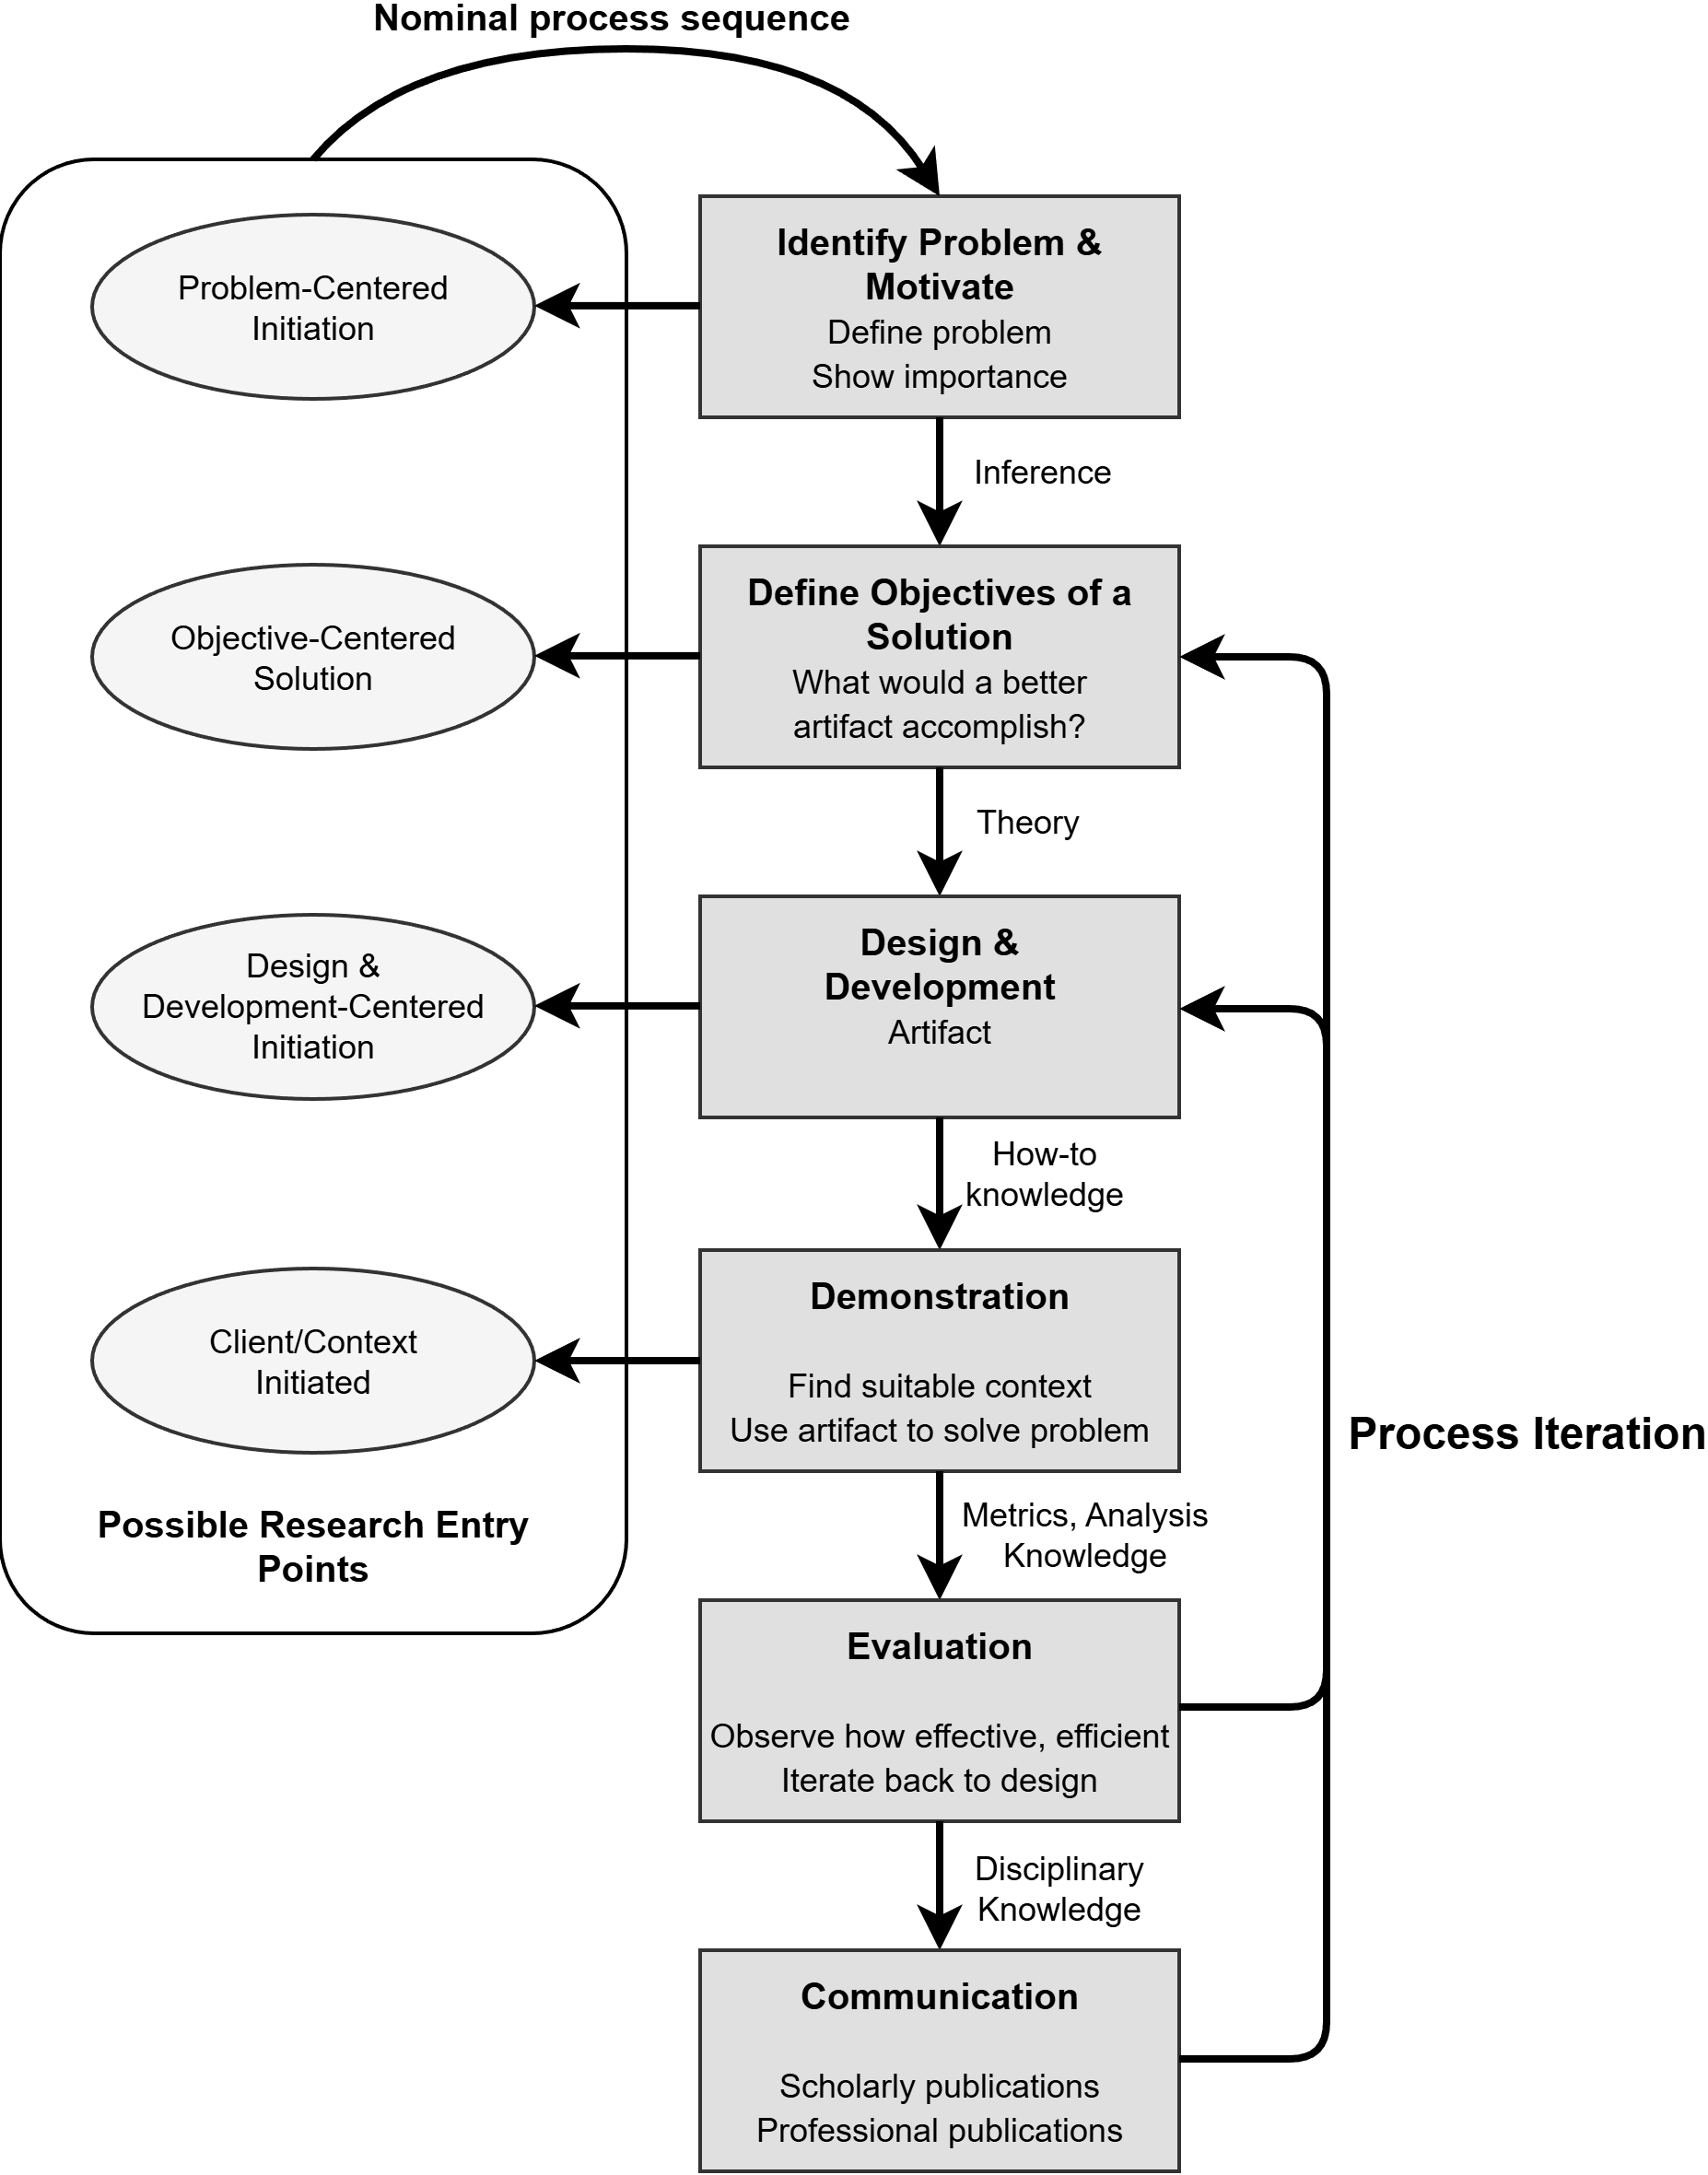
\includegraphics[width=0.95\linewidth]{figures/DSRM_Process_Model.png}
% 	\caption{DSRM Process Model \citep{peffersDesignScienceResearch2007}}
% 	\label{fig:DSRM_Process_Model}
% \end{figure}

% Problem centered initiation: Reproducibility in legacy software development projects is hard to achieve without containerization.
% So how can it be achieved with containerization?


% \begin{itemize}
% 	\item \textbf{Problem Identification:} Recognizing the need for modernization in legacy software development.
% 	\item \textbf{Objectives of a Solution:} Defining the goals for a containerized development environment.
% 	\item \textbf{Design and Development:} Developing a prototype that integrates VS Code and Docker.
% 	\item \textbf{Demonstration:} Applying the prototype in real-world scenarios.
% 	\item \textbf{Evaluation:} Assessing the effectiveness and efficiency of the solution.
% 	\item \textbf{Communication:} Presenting the findings and their implications for the field.
% \end{itemize}

% \section{Testobject}

% \section{Benchmarking Procedure}
% The evaluation will follow a defined procedure to ensure fair and consistent benchmarking:
% \begin{enumerate}
%     \item Specification of test hardware and tools to eliminate variability in performance measurements.
%     \item Development of a benchmarking suite that simulates common development tasks across various environments.
%     \item Analysis of results to identify performance trends, advantages, and limitations of each environment.
%     \item Comparison of the results to answer research questions RQ1.1 and RQ1.2.
% \end{enumerate}

% \section{Summary}
%Find reference for benchmarking
